%%%%%%%%%%%%%%%%%%%%%%%%%%%%%%%%%%%%%%%%%
% Beamer Presentation
% LaTeX Template
% Version 1.0 (10/11/12)
%
% This template has been downloaded from:
% http://www.LaTeXTemplates.com
%
% License:
% CC BY-NC-SA 3.0 (http://creativecommons.org/licenses/by-nc-sa/3.0/)
%
%%%%%%%%%%%%%%%%%%%%%%%%%%%%%%%%%%%%%%%%%

%----------------------------------------------------------------------------------------
%   PACKAGES AND THEMES
%----------------------------------------------------------------------------------------
\batchmode
\documentclass{beamer}

\mode<presentation> {

% The Beamer class comes with a number of default slide themes
% which change the colors and layouts of slides. Below this is a list
% of all the themes, uncomment each in turn to see what they look like.

%\usetheme{default}
%\usetheme{AnnArbor}
%\usetheme{Antibes}
%\usetheme{Bergen}
%\usetheme{Berkeley}
%\usetheme{Berlin}
%\usetheme{Boadilla}
%\usetheme{CambridgeUS}
%\usetheme{Copenhagen}
%\usetheme{Darmstadt}
%\usetheme{Dresden}
%\usetheme{Frankfurt}
%\usetheme{Goettingen}
%\usetheme{Hannover}
%\usetheme{Ilmenau}
%\usetheme{JuanLesPins}
%\usetheme{Luebeck}
\usetheme{Madrid}
%\usetheme{Malmoe}
%\usetheme{Marburg} 
%\usetheme{Montpellier}
%\usetheme{PaloAlto}
%\usetheme{Pittsburgh}
%\usetheme{Rochester}
%\usetheme{Singapore}
%\usetheme{Szeged}
%\usetheme{Warsaw}

% As well as themes, the Beamer class has a number of color themes
% for any slide theme. Uncomment each of these in turn to see how it
% changes the colors of your current slide theme.

%\usecolortheme{albatross}
\usecolortheme{beaver}
%\usecolortheme{beetle}
%\usecolortheme{crane}
%\usecolortheme{dolphin}
%\usecolortheme{dove}
%\usecolortheme{fly}
%\usecolortheme{lily}
%\usecolortheme{orchid}
%\usecolortheme{rose}
%\usecolortheme{seagull}
%\usecolortheme{seahorse}
%\usecolortheme{whale}
%\usecolortheme{wolverine}

%\setbeamertemplate{footline} % To remove the footer line in all slides uncomment this line
%\setbeamertemplate{footline}[page number] % To replace the footer line in all slides with a simple slide count uncomment this line

\setbeamertemplate{navigation symbols}{} % To remove the navigation symbols from the bottom of all slides uncomment this line
}

\usepackage{graphicx} % Allows including images
\usepackage{booktabs} % Allows the use of \toprule, \midrule and \bottomrule in tables
\usepackage[T1]{fontenc}
\usepackage{lmodern}
\usepackage{epsf}
\usepackage{hyperref}
\usepackage{caption}
\usepackage{subcaption}



% \newcounter{eqn}
% \renewcommand*{\theeqn}{\alph{eqn})}
% \newcommand{\num}{\refstepcounter{eqn}\text{\theeqn}\;}



%----------------------------------------------------------------------------------------
%   TITLE PAGE
%----------------------------------------------------------------------------------------

\title[Uniformity: metrics and classifiers]{New approaches for boosting to uniformity} % The short title appears at the bottom of every slide, the full title is only on the title page
\author[Alex Rogozhnikov]{
\underline{Alex Rogozhnikov}$^{a,b}$,
Aleksandar Bukva$^c$, 
Vladimir Gligorov$^d$,
Andrey Ustyuzhanin$^{b,e,f}$ and
Mike Williams$^g$
}

%\institute[SINP MSU] % Your institution as it will appear on the bottom of every slide, may be shorthand to save space

\institute[]{
$^a$  Lomonosov Moscow State University, Moscow\\
$^b$  Yandex School of Data Analysis, Moscow\\
$^c$  Faculty of Physics, Belgrade \\
$^d$  Organisation Europ\'eenne pour la Recherche Nucl\'eaire (CERN), Geneva  \\
$^e$  Moscow Institute of Physics and Technology, Moscow\\
$^f$  Imperial College, London\\
$^g$  Massachusetts Institute of Technology, Cambridge 
\medskip
\\
\textit{alex.rogozhnikov@yandex.ru} % Your email address
}
\date{11 November, 2014}

\begin{document}
\begin{frame}
\titlepage % Print the title page as the first slide
\end{frame}


%\begin{frame}
%\frametitle{Overview} % Table of contents slide, comment this block out to remove it
%\tableofcontents % Throughout your presentation, if you choose to use \section{} and \subsection{} commands, these will automatically be printed on this slide as an overview of your presentation
%\end{frame}

%   PRESENTATION SLIDES





\def\knn{\text{knn}}
\def\knni{\text{knn}(i)}
\newcommand{\abs}[1]{\left\vert#1\right\vert}
\newcommand{\sgn}{\operatorname{sgn}}

\def\bineff{\text{eff}_\text{bin}}
\def\binweight{\text{weight}_\text{bin}}
\def\globaleff{\text{eff}}
\def\SDE{\text{SDE}}
\def\bin{\text{bin}}
\def\theil{\text{Theil}}
\def\score{\text{score}}
\def\knn{\text{knn}}
\def\FL{\text{FL}}
\def\AdaLoss{L_\text{ada}}
\def\knnAdaLoss{L_\text{knn-ada}}
\def\generalAda{L_\text{general}}


\begin{frame}
    \frametitle{Outline}
    \begin{itemize}
    \item What is uniformity (of predictions)? 
    \item How to measure it? 
    \item How to achieve it? (classifiers proposed)
    \end{itemize}
\end{frame}

\begin{frame}
    \frametitle{Uniformity}
    In particle physics, apart from optimizing some FOM of classifier (BDT, ANN), 
    there are cases when we want to have uniformity of predictions
    \begin{itemize}
    \item Dalitz-plot analysis (or any angular or amplitude analysis)

    \item search for a new particle (not to get fake peak)

    \item sensitivity for new signal 
        in wide range of mass (lifetime ...), \\
        ({\small i.e. train only one classifier, not separate for each mass})

    \end{itemize}
    $ $

    \textbf{Uniform variables} --- variables, along which uniformity of selection is desired (Dalitz variables, mass variable).
    \bigskip \\
    Typical solution: choose such features which don't give an ability to reconstruct 'mass' (or other selected 'uniform variables').
\end{frame}

\begin{frame}
    \frametitle{What is uniformity?}

    Predictions of some classifier are called \textit{uniform} in variables $var_1, \dots, var_n$ if prediction and set of this variables is \textit{statistically independent}. 

    This (and only this) guarantees that any cut of prediction of classifier will produce the same efficiency in every region over $var_1, \dots, var_n$

    % definition of uncorrelated variables
    \pause
    % picture with absolutely uniform predictions
    % left bottom right top
	% picture with skew

    \begin{figure}
        \centering
        \begin{subfigure}[b]{0.48\textwidth}
            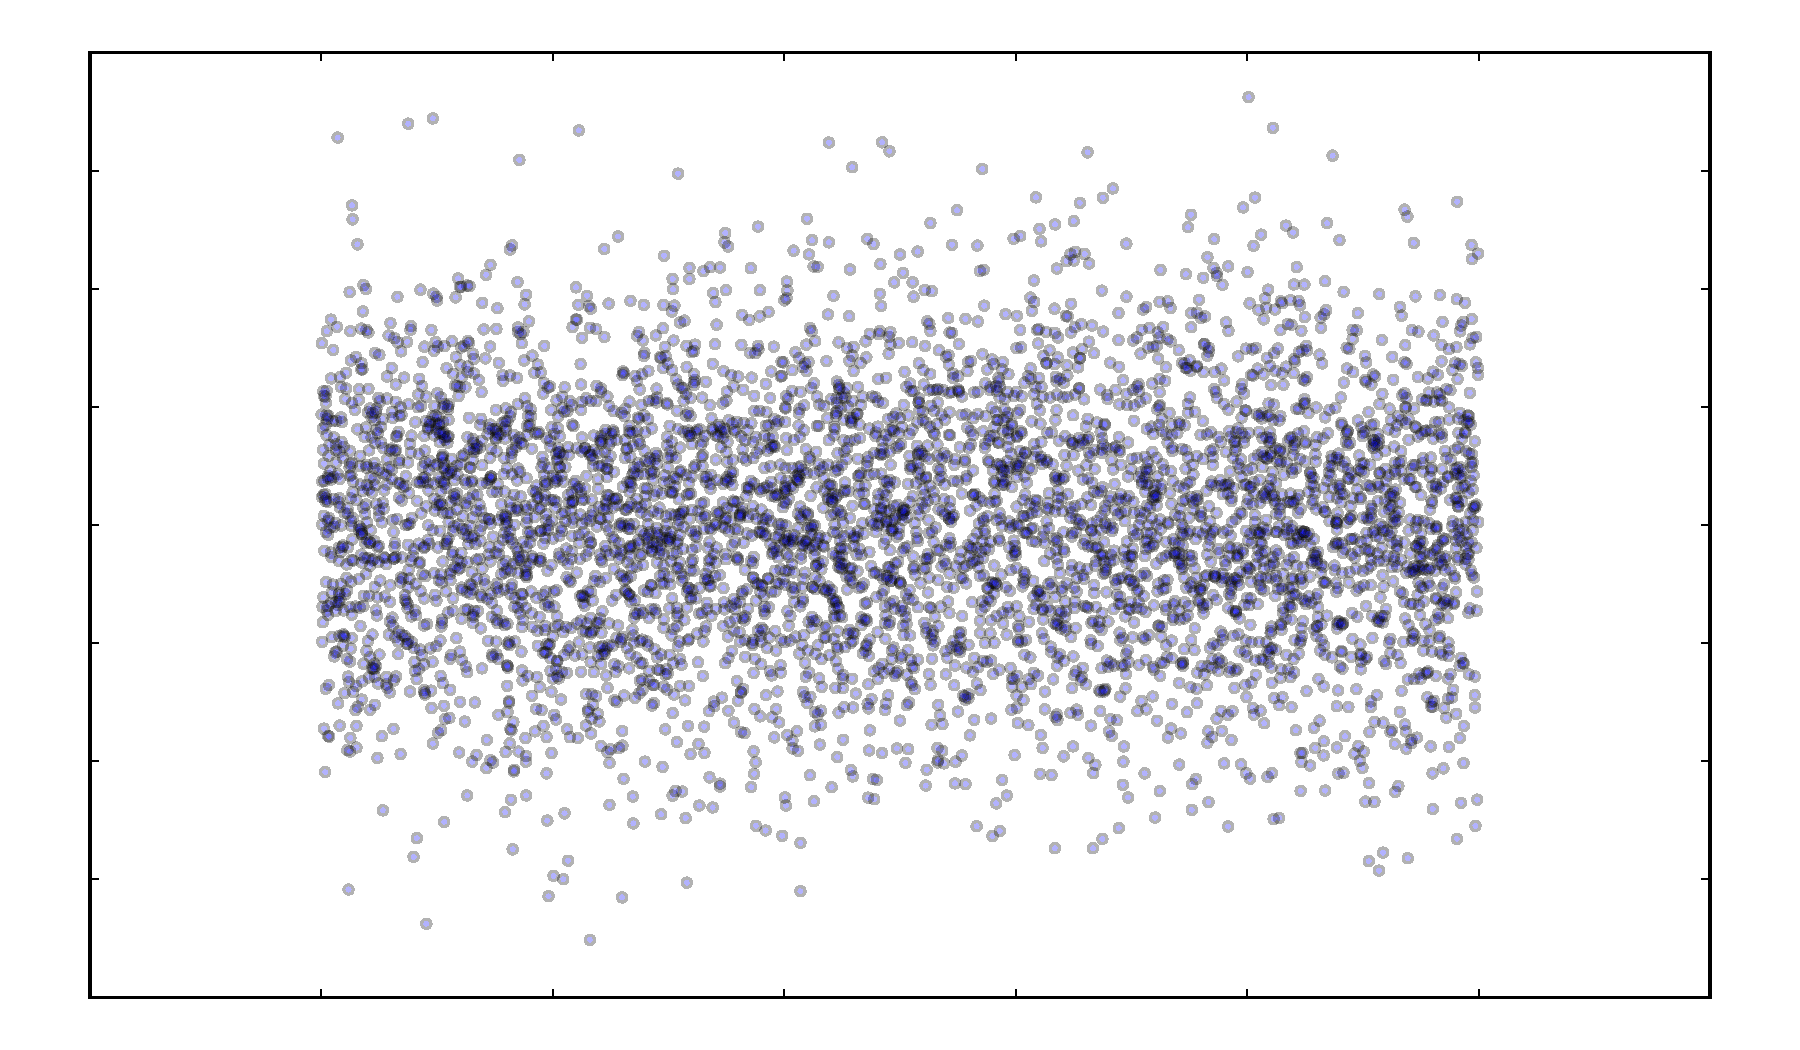
\includegraphics[width=\textwidth, height=4cm]{img/uniform.pdf}
            \caption{Uniform predictions}
        \end{subfigure}
        \begin{subfigure}[b]{0.48\textwidth}
            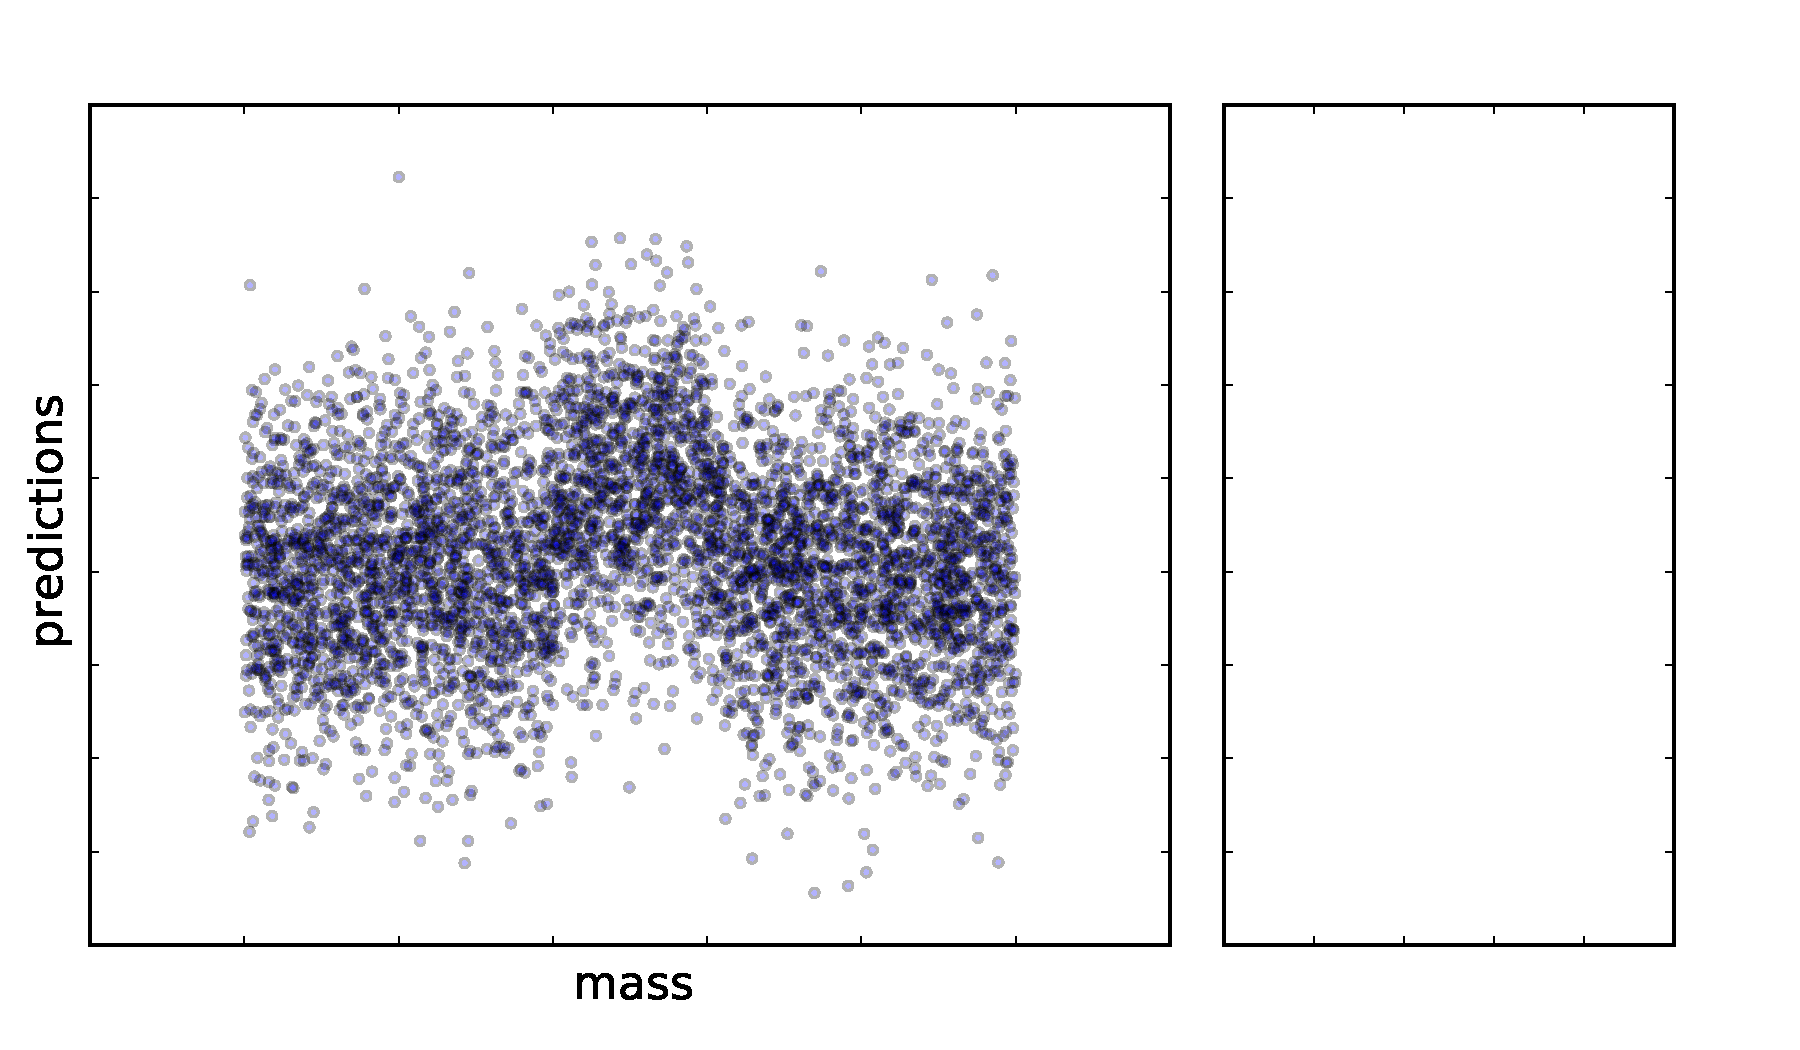
\includegraphics[width=\textwidth, height=4cm]{img/nonuniform.pdf}
            \caption{Non-uniform}
        \end{subfigure}
    \end{figure}

\end{frame}

\begin{frame}
    \frametitle{Boosting to uniformity}
    % TODO link
    Previous work: \textbf{uBoost} \\
    {\small J. Stevens and M. Williams,
        {\em uBoost: A boosting method for producing uniform selection efficiencies from multivariate classifiers}, 
        JINST {\bf 8}, P12013 (2013). [arXiv:1305.7248]
    }
    \bigskip \\
    % The classifiers we propose alter the \textbf{boosting} procedure as well

    \center
    \includegraphics[width=0.7\textwidth]{img/uboost.png}

    In this talk I present alternate methods for producing BDTs with uniform selection efficiency.
\end{frame}

\begin{frame}[t]
    \frametitle{Boosting: Gradient Boosting with plain AdaLoss}
    Gradient boosting on trees is widely used algorithm, 
    it's built upon decision tree regressors with usage of some loss function. 

    Usual AdaLoss ($y_i = +1$ for signal, $-1$ for background):
    \[
        \AdaLoss = \sum_{i \in \text{events}} \exp [- \score_i \, y_i] 
    \]

    Gradient boosting tries to minimize the loss function by 'steepest descent'-like procedure.

    Pseudo-residual of AdaLoss:
    \[
        -\dfrac{\partial \, \AdaLoss}{\partial \, \score_i} = y_i \exp[- \score_i \, y_i],
    \]

    We need to introduce some loss, which penalizes non-unifomity.

\end{frame}

\begin{frame}
    \frametitle{Similarity-based approach for measuring uniformity}
    Idea: uniformity means that distribution of predictions in every bin is equal. 
    \bigskip \\ 
    {\small
  	Let's compare the global distribution (blue hist) 
  	with distibution in one bin (yellow hist).
  	Yellow rectangle shows the events in selected bin over mass.
  	}

    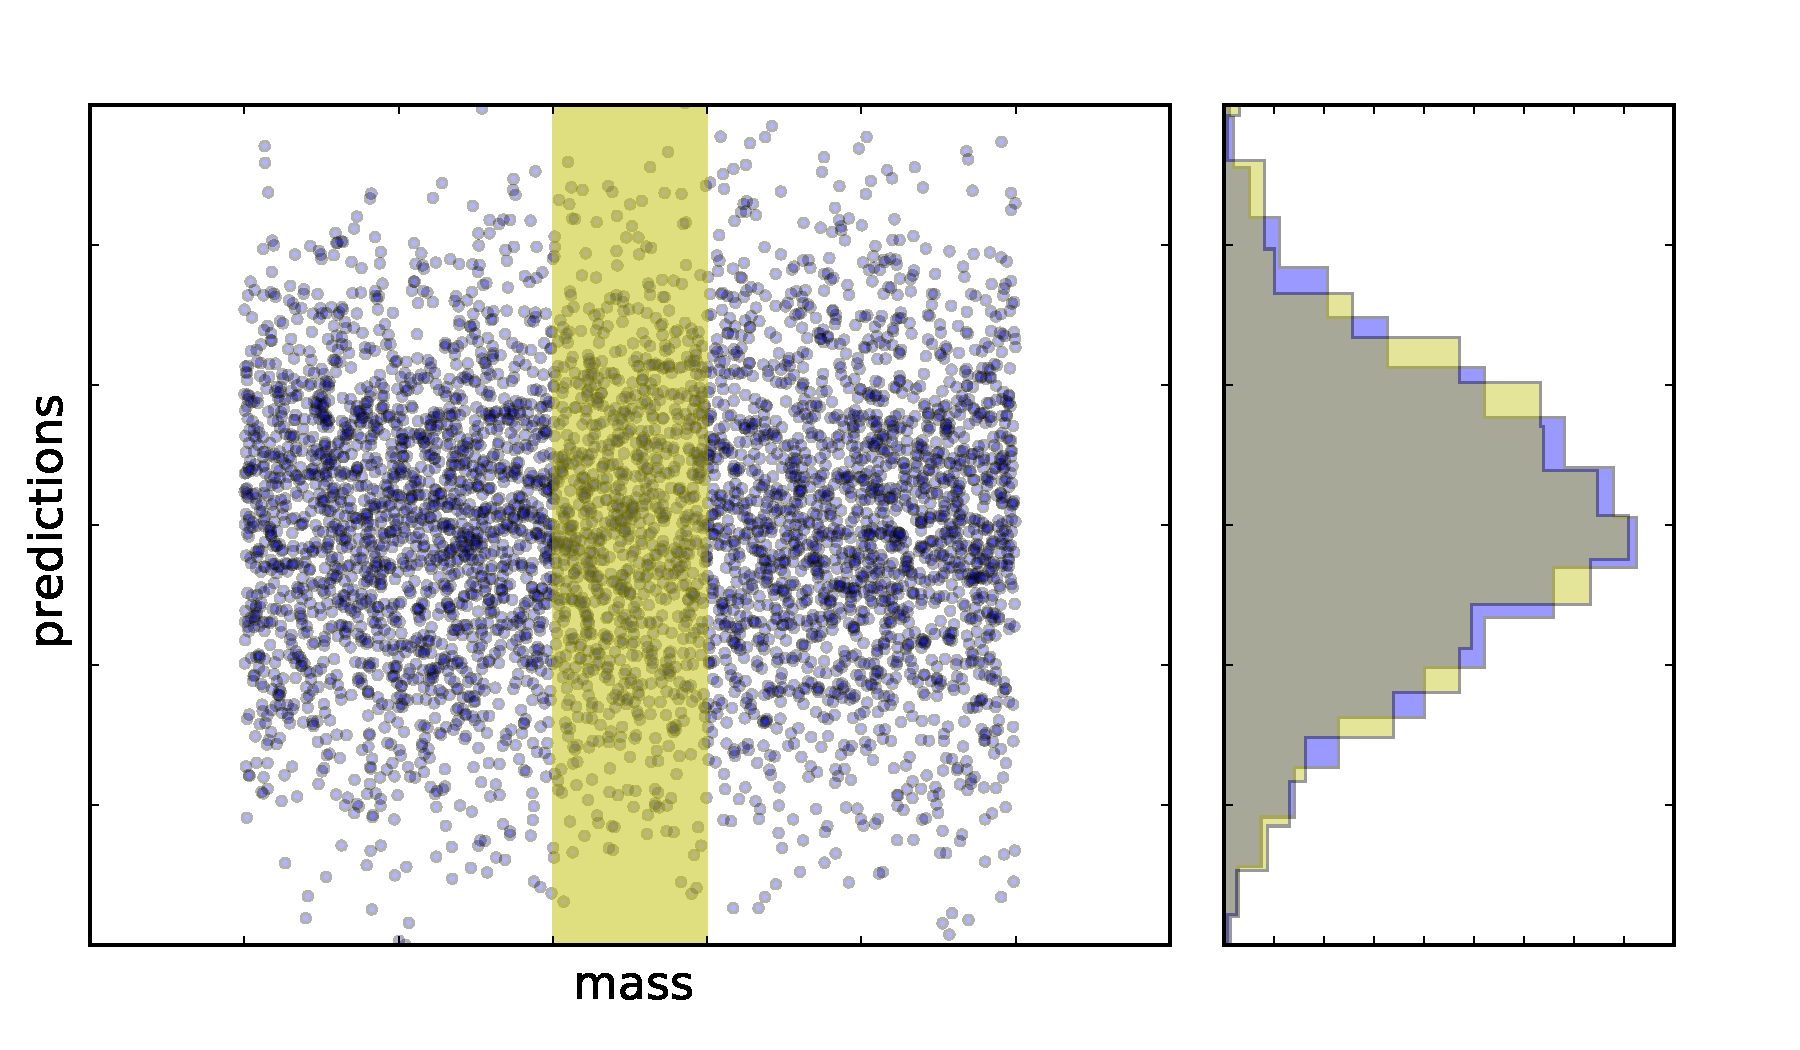
\includegraphics[width=0.5\textwidth, height=4cm]{img/uniform_hist.pdf}
    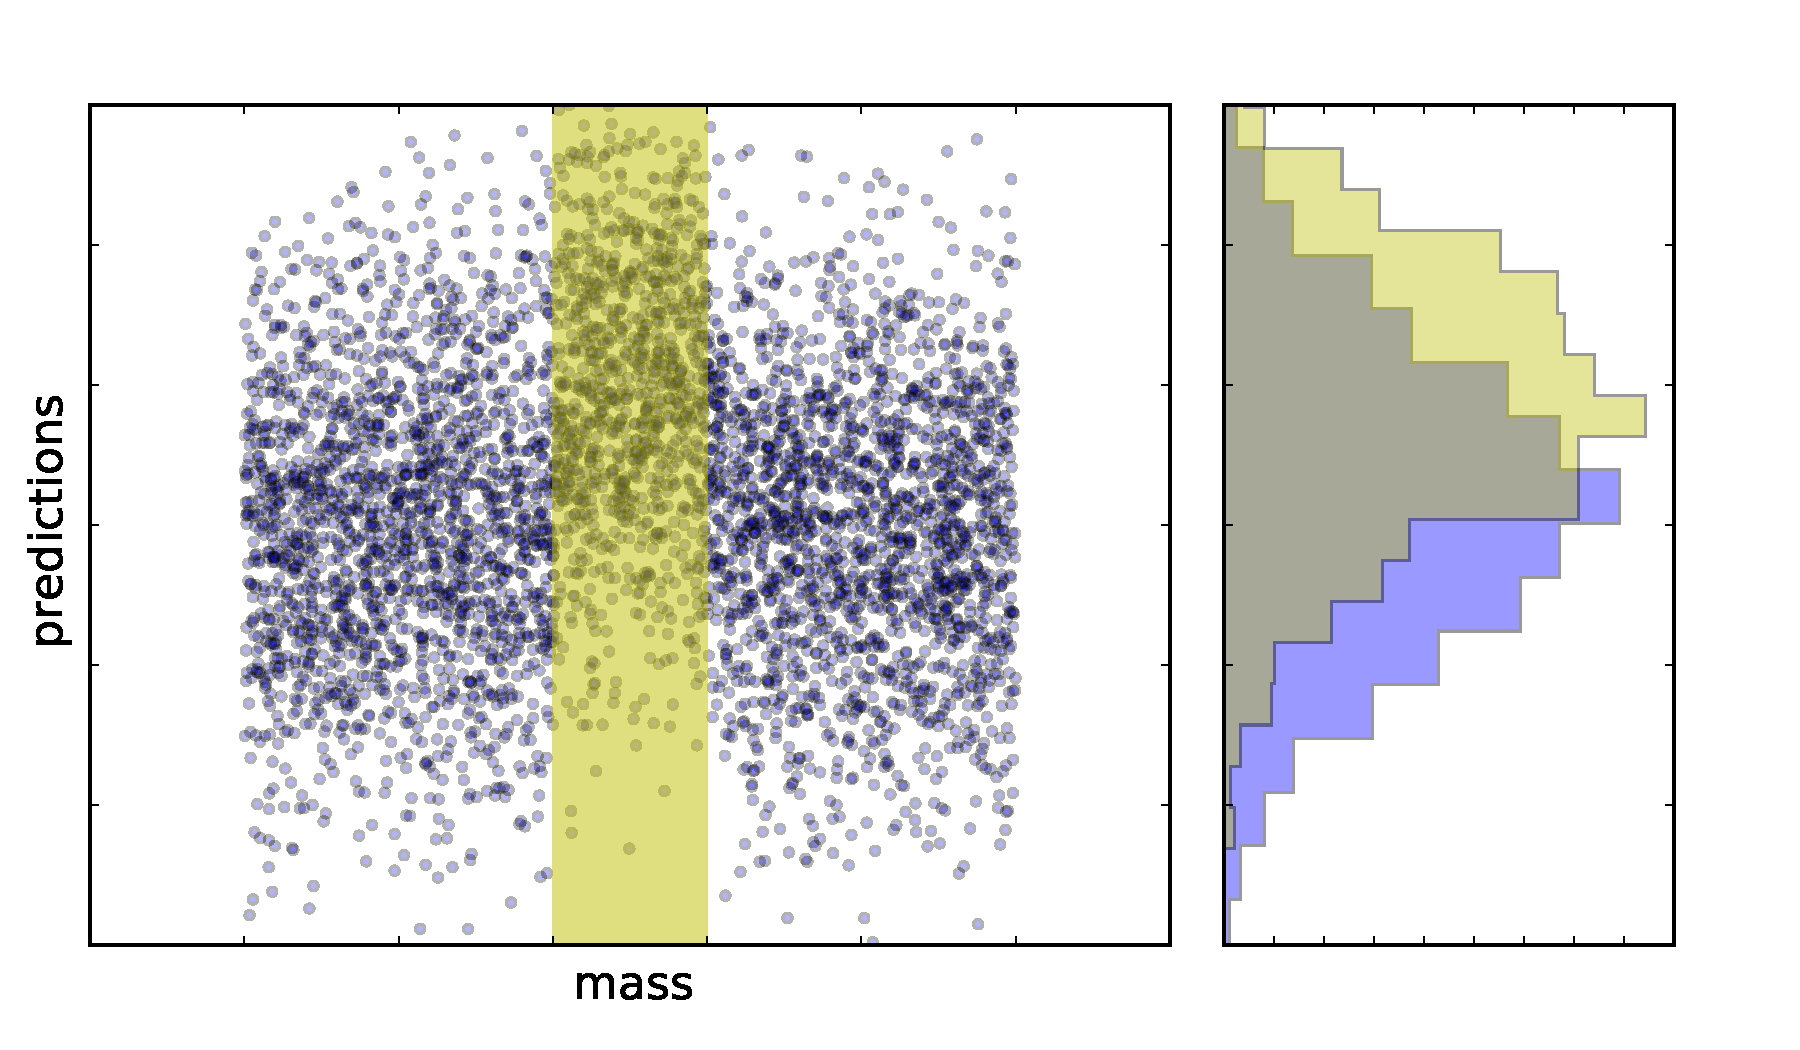
\includegraphics[width=0.5\textwidth, height=4cm]{img/nonuniform_hist.pdf}    

\end{frame}

\begin{frame}[t]
    \frametitle{Similarity-based approach}

    Let $F(x) = \text{P}(prediction < x)$ --- cdf of all predictions, \\
    $F_{\bin}(x) = \text{P}(prediction \; in \; \text{bin} < x)$ --- cdf of predictions in bin over mass. Define $\binweight = \frac{\text{weight of events in bin}}{\text{weight of all events}}$ 
    \bigskip \\

    % $\binweight$ --- weights of bins.

    Kolmogorov-Smirnov measure (uninformative)
    \[
    	\sum_{\bin} \binweight \max_x \abs{F_{\bin}(x) - F(x)},
    \]
    Cram\'er--von Mises similarity
    \[
    	 \sum_{\bin} \binweight \int \abs{F_{\bin}(x) - F(x)}^p dF(x)
    \]
\end{frame}

\begin{frame}[t]
    \frametitle{Boosting: Gradient Boosting with FlatnessLoss (uGBFL)}
    CvM measure of non-uniformity:
    \[
        \sum_{\bin} \binweight \int \abs{F_{\bin}(x) - F(x)}^p dF(x),
    \]
    Let's modify this function:
    \[
        \FL = \sum_{\bin} \binweight \int \abs{F_{\bin}(x) - F(x)}^p {\textcolor{red}{dx}}
    \]
    so that it becomes differentiable
    \[
        \dfrac{\partial} {\partial \, \score_i} \FL
        \cong 
        w_i \, p \,  \abs{F_{\bin(i)}(x) - F(x)}^{p-1}
        \sgn[F_{\bin(i)}(x) - F(x)]
        \Bigg|_{x=\score_i}
    \]
\end{frame}

\begin{frame}
    \frametitle{Boosting: Gradient Boosting with FlatnessLoss (uGBFL)}

    FL doesn't take into account the quality of predictions, only uniformity. 

    So what we use in practice is linear combination of FlatnessLoss and AdaLoss:
    \[
        \text{loss} = \FL + \alpha \, \AdaLoss
    \]

    First one penalizes non-uniformity, second one --- poor predictions, 
    $\alpha$ is usually taken small.

\end{frame}

\begin{frame}[t]
    \frametitle{Boosting: Gradient Boosting with \textit{knn}AdaLoss (uGBkNNAdaLoss) }
    As another approach we define:\textit{kNN}AdaLoss:
    \[
        \knnAdaLoss = \sum_{i \in events} \exp[-y_i \times \sum_{j \in \text{knn}(i)} \score_j],
    \]
    It can be written as particular case of:
    \[
        \generalAda = \sum_i \exp [- y_i \sum_j a_{ij} \, \score_j ],
    \]
    \[
        a_{ij} = 
        \begin{cases} 
            1, & j \in \knn(i), \text{ events $i$ and $j$ belong to the same class} \\
            0, & \text{otherwise},
        \end{cases}
    \]

    This is one particular choice of $a_{ij}$; \\
    in general case matrix $a_{ij}$ even may be non-square.

\end{frame}

\begin{frame}[t]
    \frametitle{\textit{knn}AdaBoost}
    Usual AdaBoost reweighting procedure ($p_i$ is prediction of last classifier):
    \[
        w_i' = w_i \times \exp[-y_i \, p_i],
    \]

    \textit{knn}AdaBoost uses mean of predictions of neighbours 
    \[
        w_i' = w_i \times \exp[-y_i \, \dfrac{1}{k} \sum_{j \in \knni} p_j]
    \]
    (neighbours are of the same class).

    Thus boosting focuses not on the events that were poorly classified, but on the regions with poor classification.
\end{frame}

% \begin{frame}[t]
%     \frametitle{Boosting: Gradient Boosting with \textit{knn}AdaLoss }
%     Gradient boosting on trees is widely used algorithm, 
%     it's built upon decision tree regressors with usage of some loss function. 

%     Usual AdaLoss:
%     \[
%         \AdaLoss = \sum_{i \in \text{events}} w_i \times \exp [- \score_i \, y_i] 
%     \]
%     Pseudo-residual of AdaLoss:
%     \[
%         -\dfrac{\partial \, \AdaLoss}{\partial \, \score_i} = w_i \, y_i \exp[- \score_i \, y_i],
%     \]
%     \textit{knn}AdaLoss:
%     \[
%         \knnAdaLoss = \sum_{i \in events} \exp[-y_i \times \sum_{j \in \text{knn}(i)} \score_j],
%     \]

% \end{frame}


\begin{frame}[t]
    \frametitle{Example analysis: distibutions}

    \begin{figure}[] 
          \centering 
          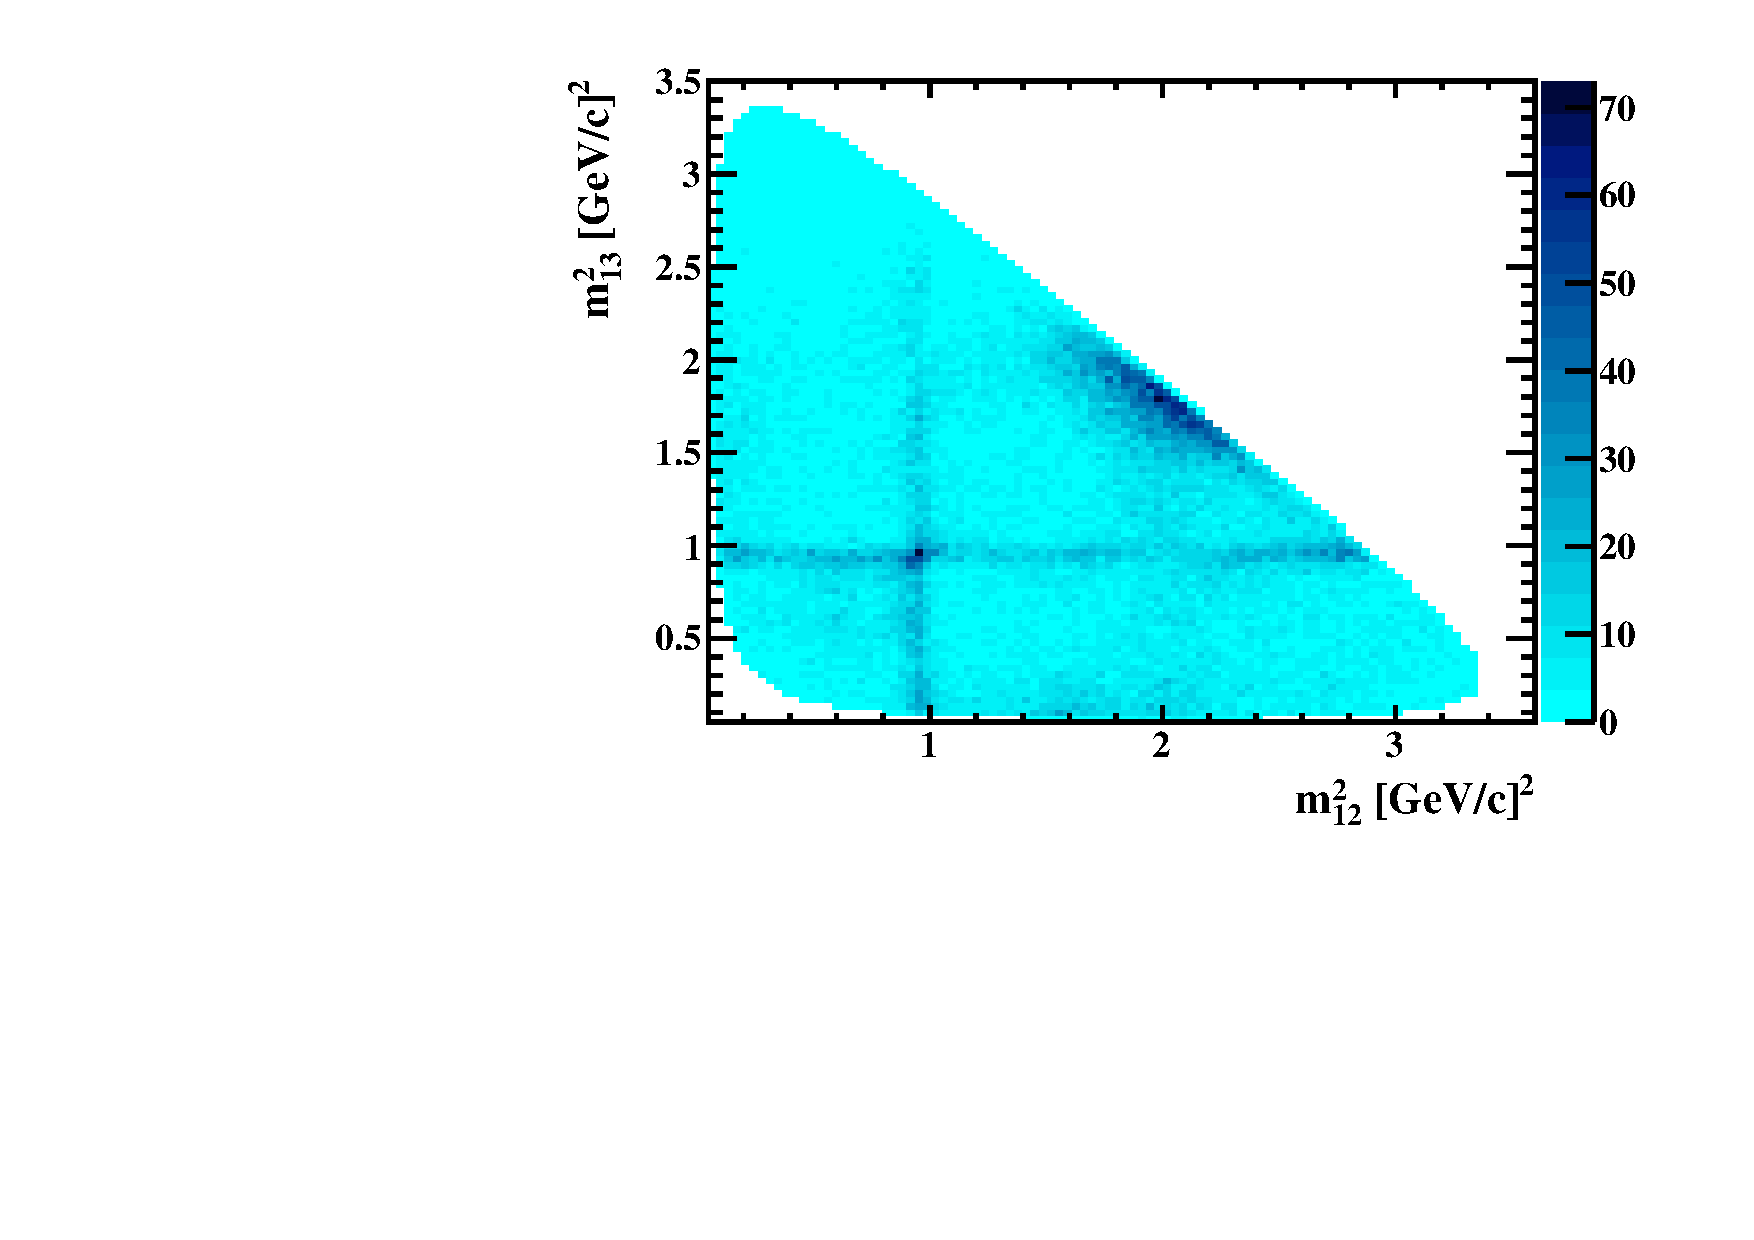
\includegraphics[width=0.49\textwidth]{../paperdraft/graphs2/DP_sig.pdf}
          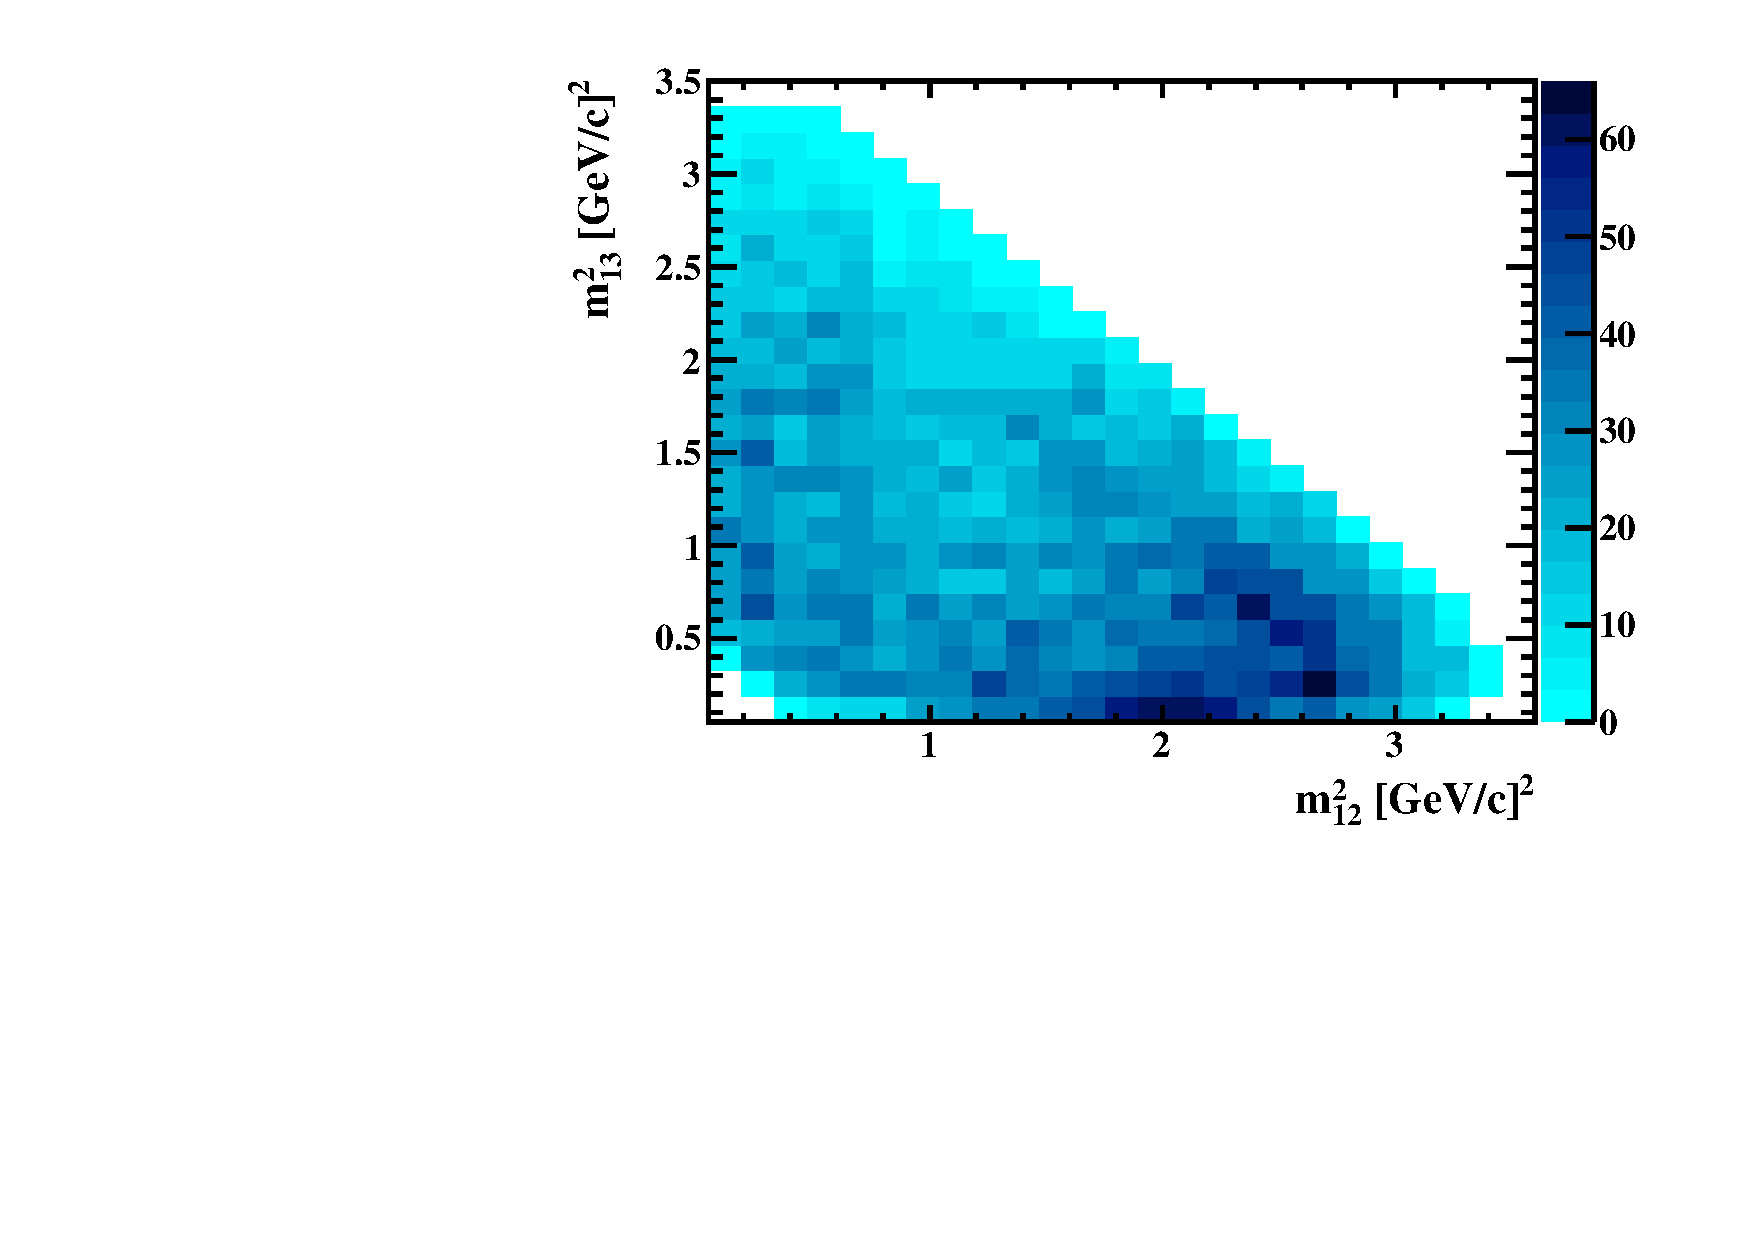
\includegraphics[width=0.49\textwidth]{../paperdraft/graphs2/DP_bkgd.pdf}
    \end{figure}
    Dalitz-plot distributions for (left) signal and (right) background for the $D_s^\pm\to\pi^+\pi^-\pi^\pm$.  The three pions are labeled here as 1, 2 and 3 and ordered according to increases momentum.
\end{frame}

\begin{frame}[t]\frametitle{Abbreviations}
    \begin{table}
      \begin{center}
        \caption{\label{tab:algs} Description of uniform boosting algorithms.}
        \begin{tabular}{c|c}
          %\toprule
          \hline
          Name & Description \\
          \hline
          %\midrule
            uBoost & algorithm introduced in [arXiv:1305.7248]\\
          \hline
          %\midrule 
            kNNAda & AdaBoost modification using averaging over knn \\
            uGBkNN & gradient boost using kNNAdaLoss loss function \\
            uGBFL(bin) & gradient boost using flatness loss $+ \alpha$ AdaLoss  \\
            uGBFL(kNN) & same except kNN events are used rather than bins \\
          \hline
          %\bottomrule
        \end{tabular}
      \end{center}
    \end{table}

\end{frame}


\begin{frame}[t]
    \frametitle{Example analysis}
    \begin{figure}[] 
        \centering 
        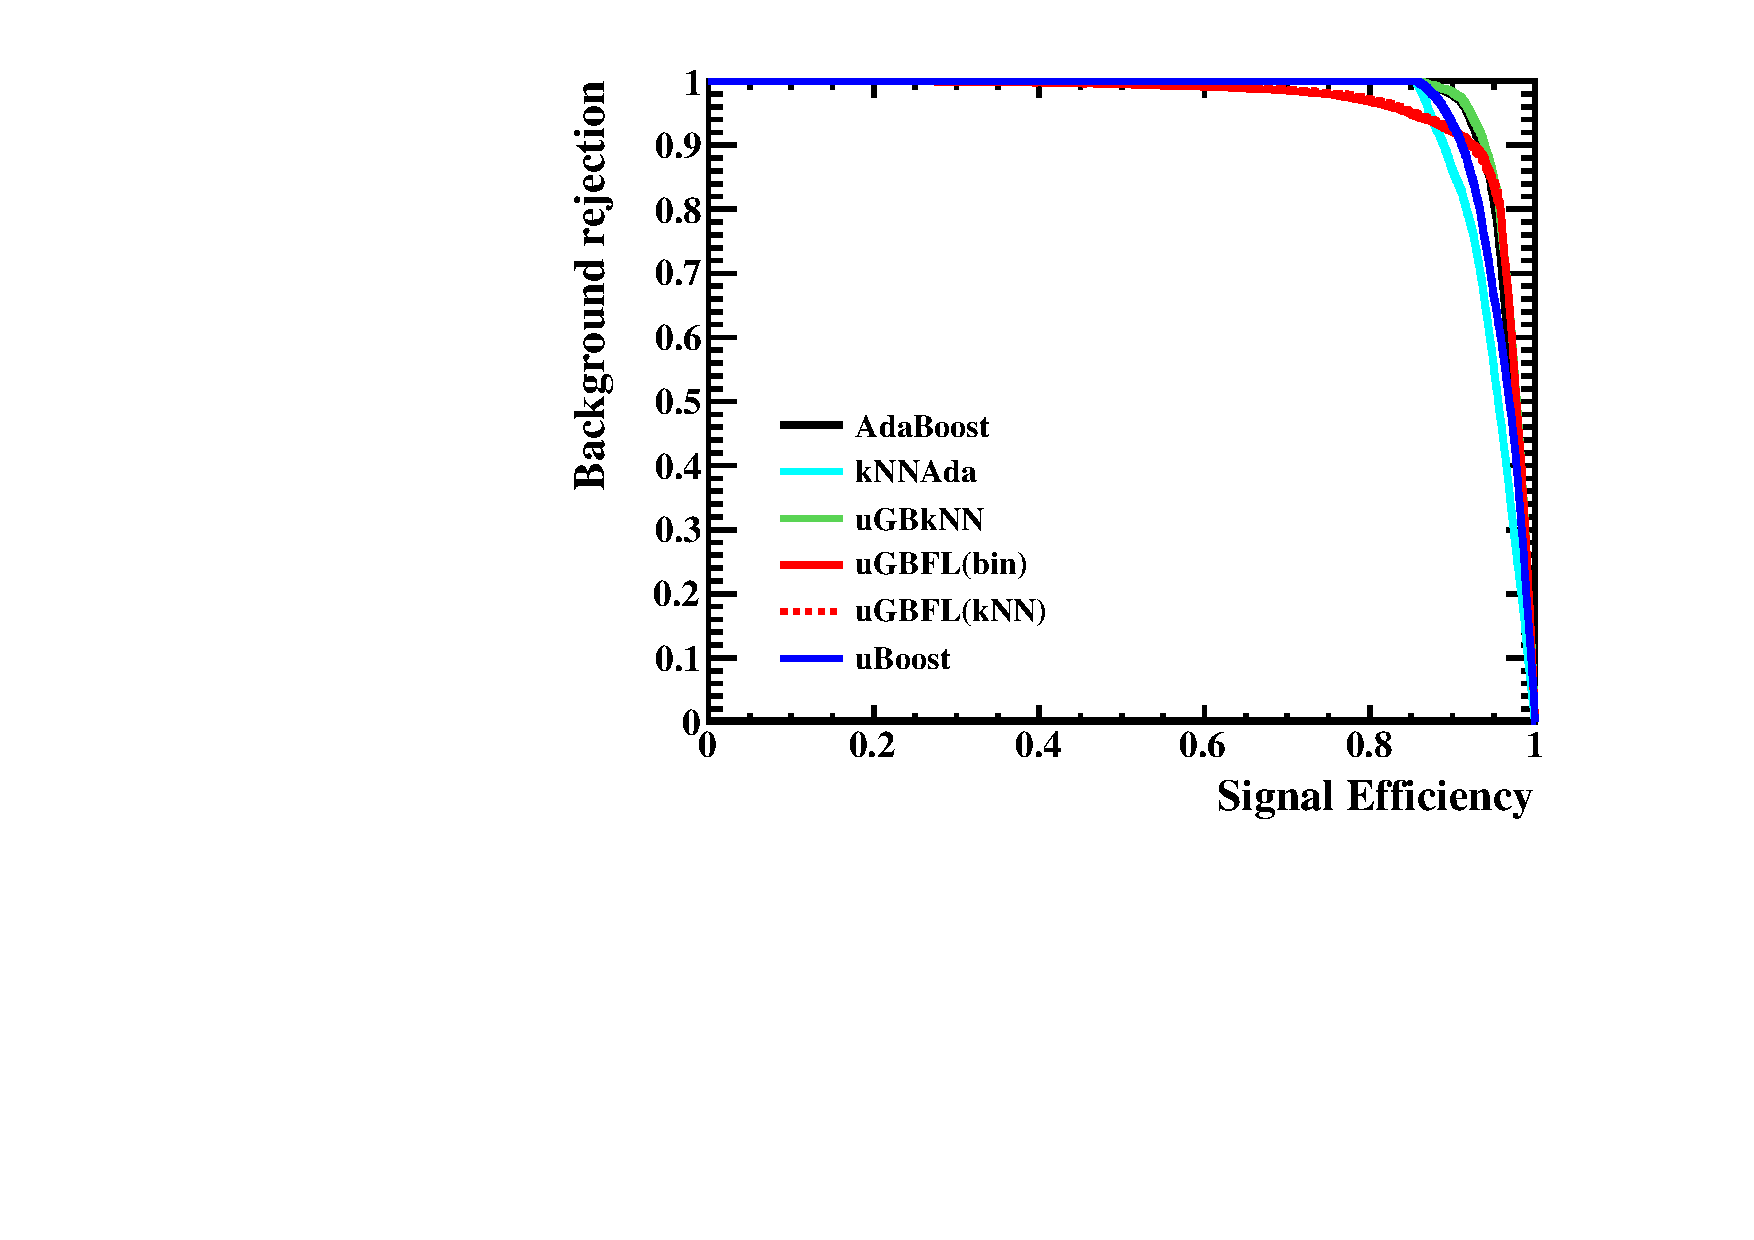
\includegraphics[width=0.49\textwidth]{../paperdraft/graphs2/ROC_DP.pdf}
        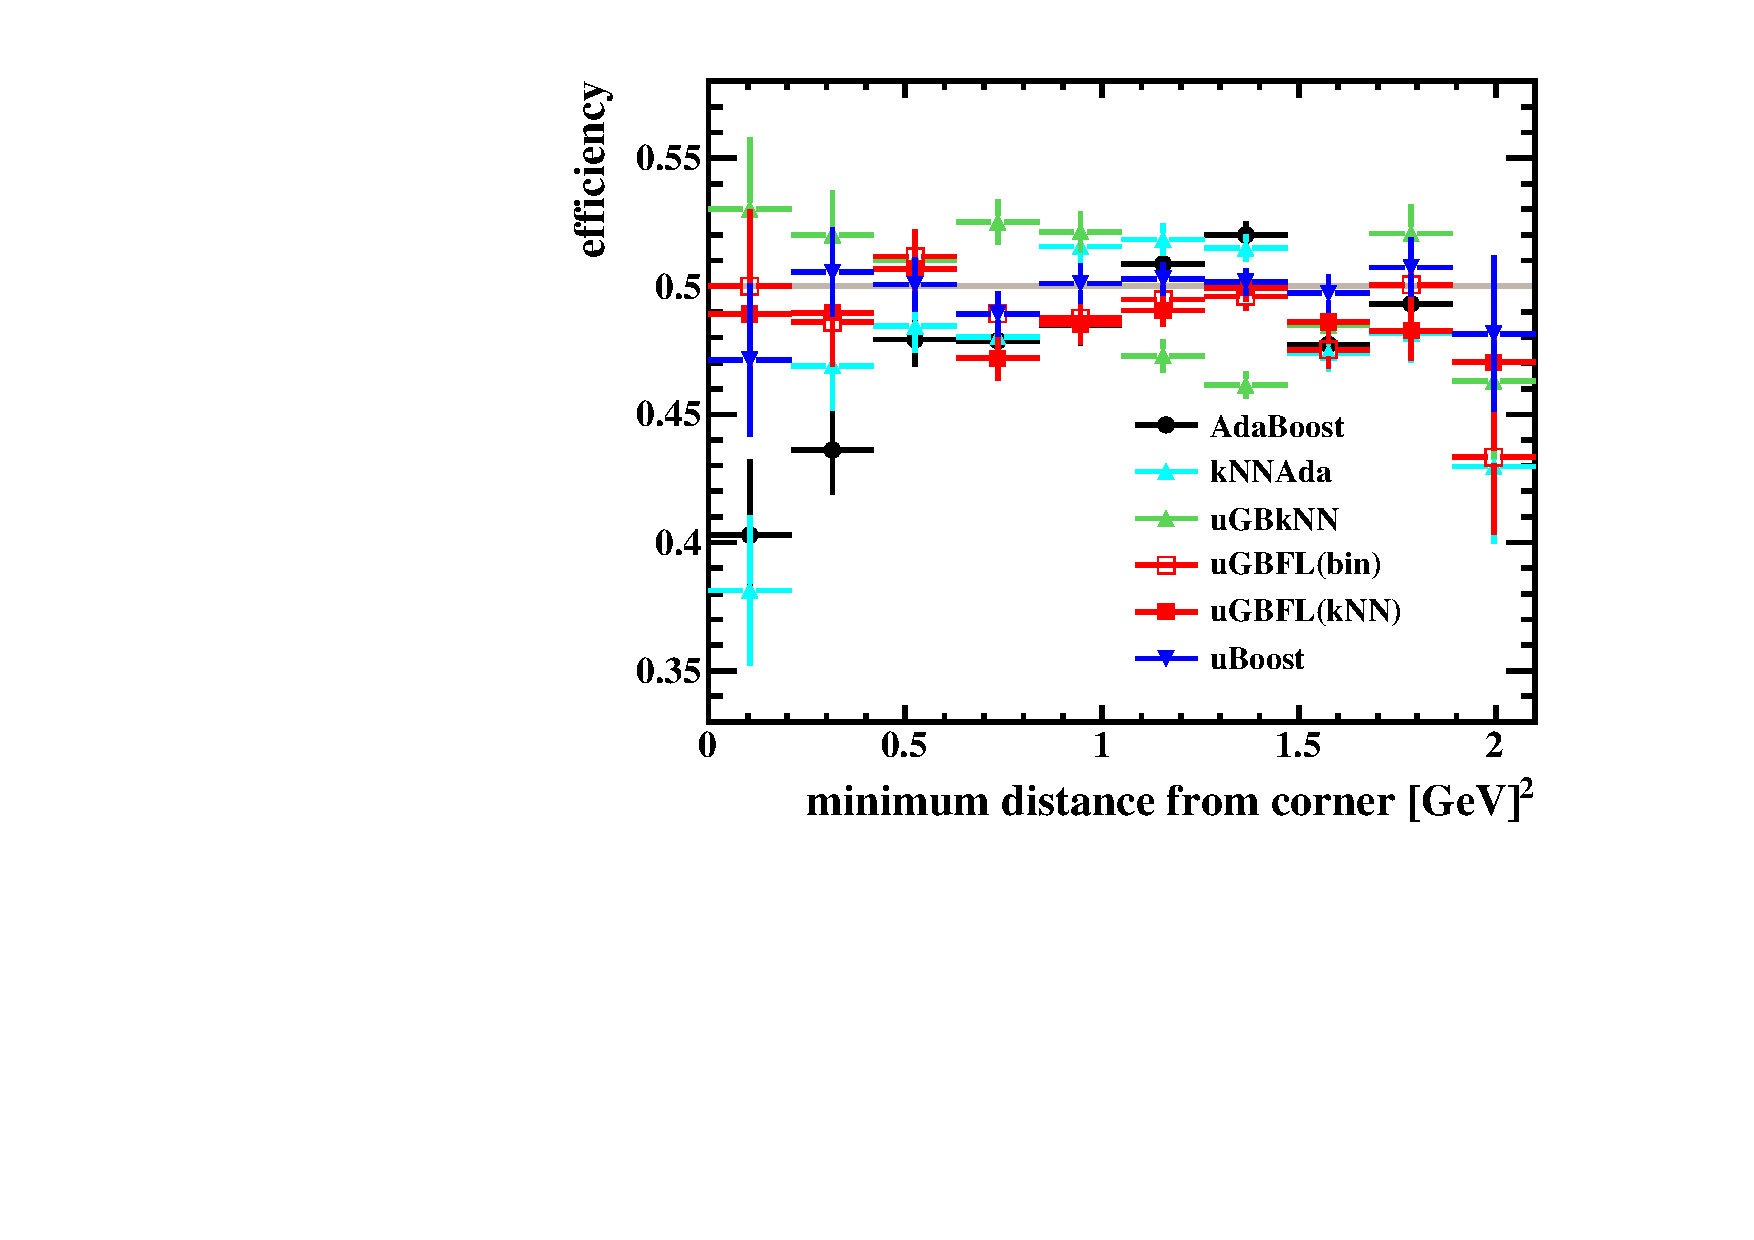
\includegraphics[width=0.49\textwidth]{../paperdraft/graphs2/DP_compare.pdf}
        \\
    \end{figure}

    (left) ROC curves for classifiers. \\
    (right) Efficiency {\em vs} distance to a corner of the Dalitz-plot.  An arbitrary working point of 50\% integrated efficiency is displayed. 
    \bigskip \\
    AdaBoost produces a much lower efficiency near corners of Dalitz plot, while uGBFL and uBoost are consistent with flat.
\end{frame}


\begin{frame}[t]
    \frametitle{Example analysis, tradeoff }
    Increasing of $\alpha$ parameter in uGBFL results in better quality of classification, but less uniformity of predictions.

    \begin{figure}[] 
        \centering 
        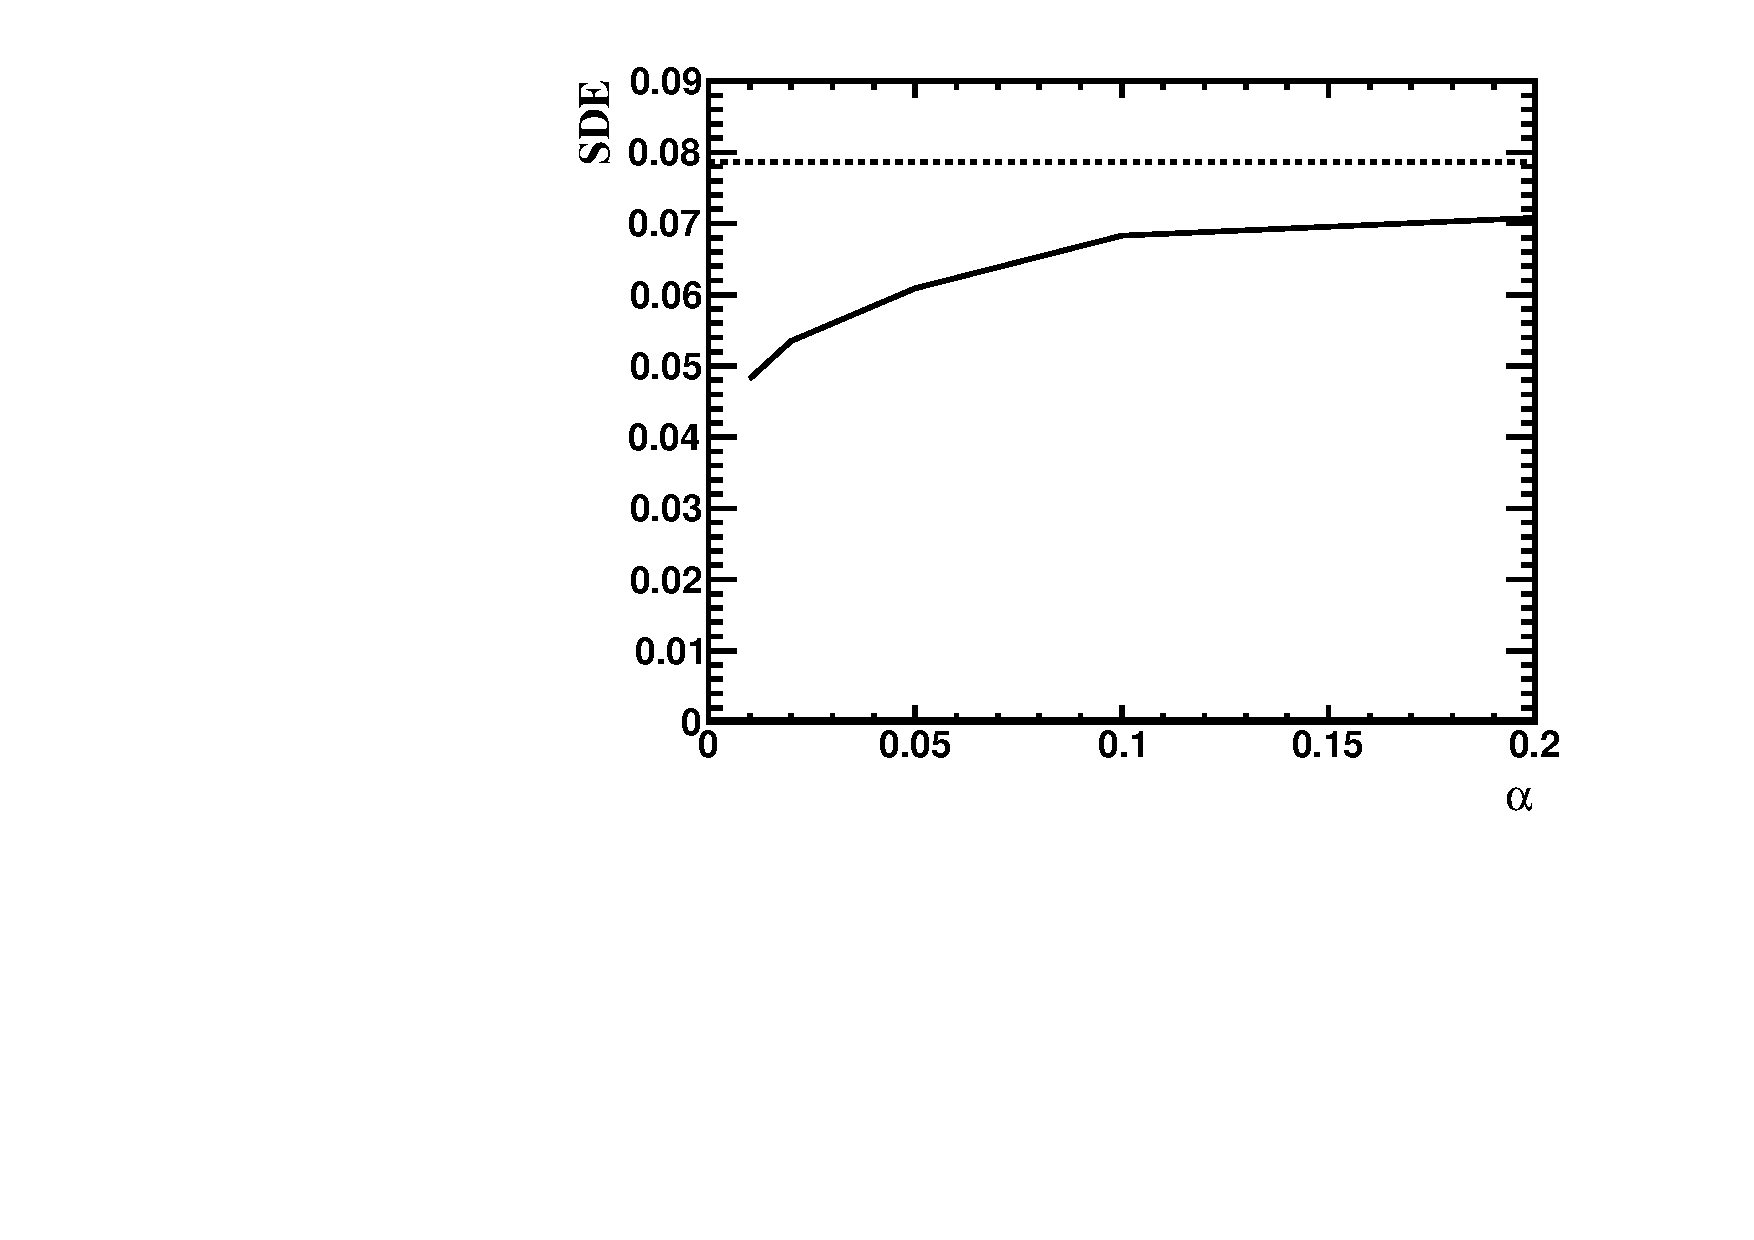
\includegraphics[width=0.49\textwidth]{../paperdraft/graphs2/sde_v_alpha.pdf}
        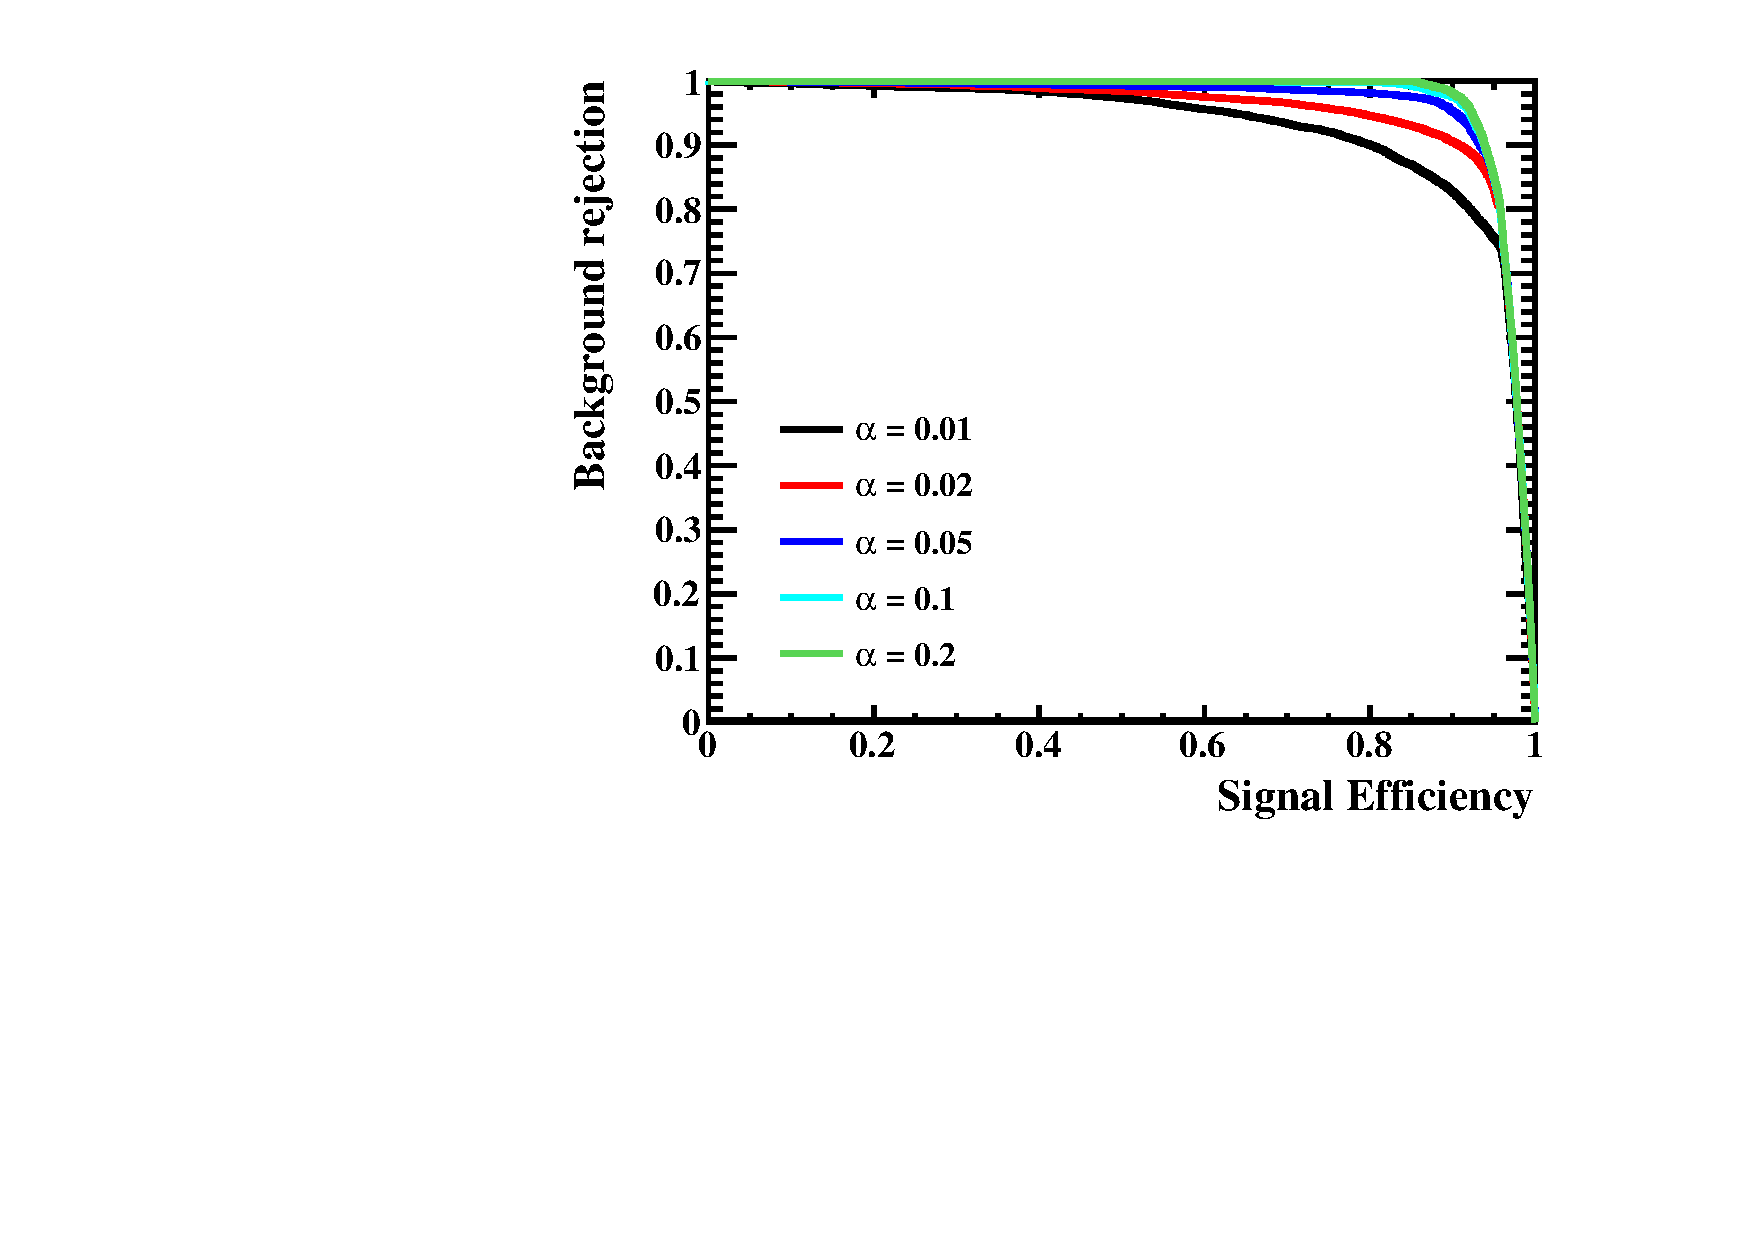
\includegraphics[width=0.49\textwidth]{../paperdraft/graphs2/ROC_DP_Alpha.pdf}
    \end{figure}
    (left) SDE for uGBFL(bin) for different values of $\alpha$, \\
    SDE = Standard Deviation of Efficiency (0 = perfectly uniform).
    \medskip    \\
    (right) ROC curves for uGBFL(bin) for different values of $\alpha$.

\end{frame}


\begin{frame}[t]
    \frametitle{Example analysis 2: training on mass sideband}

    \begin{figure}[] 
        \centering 
        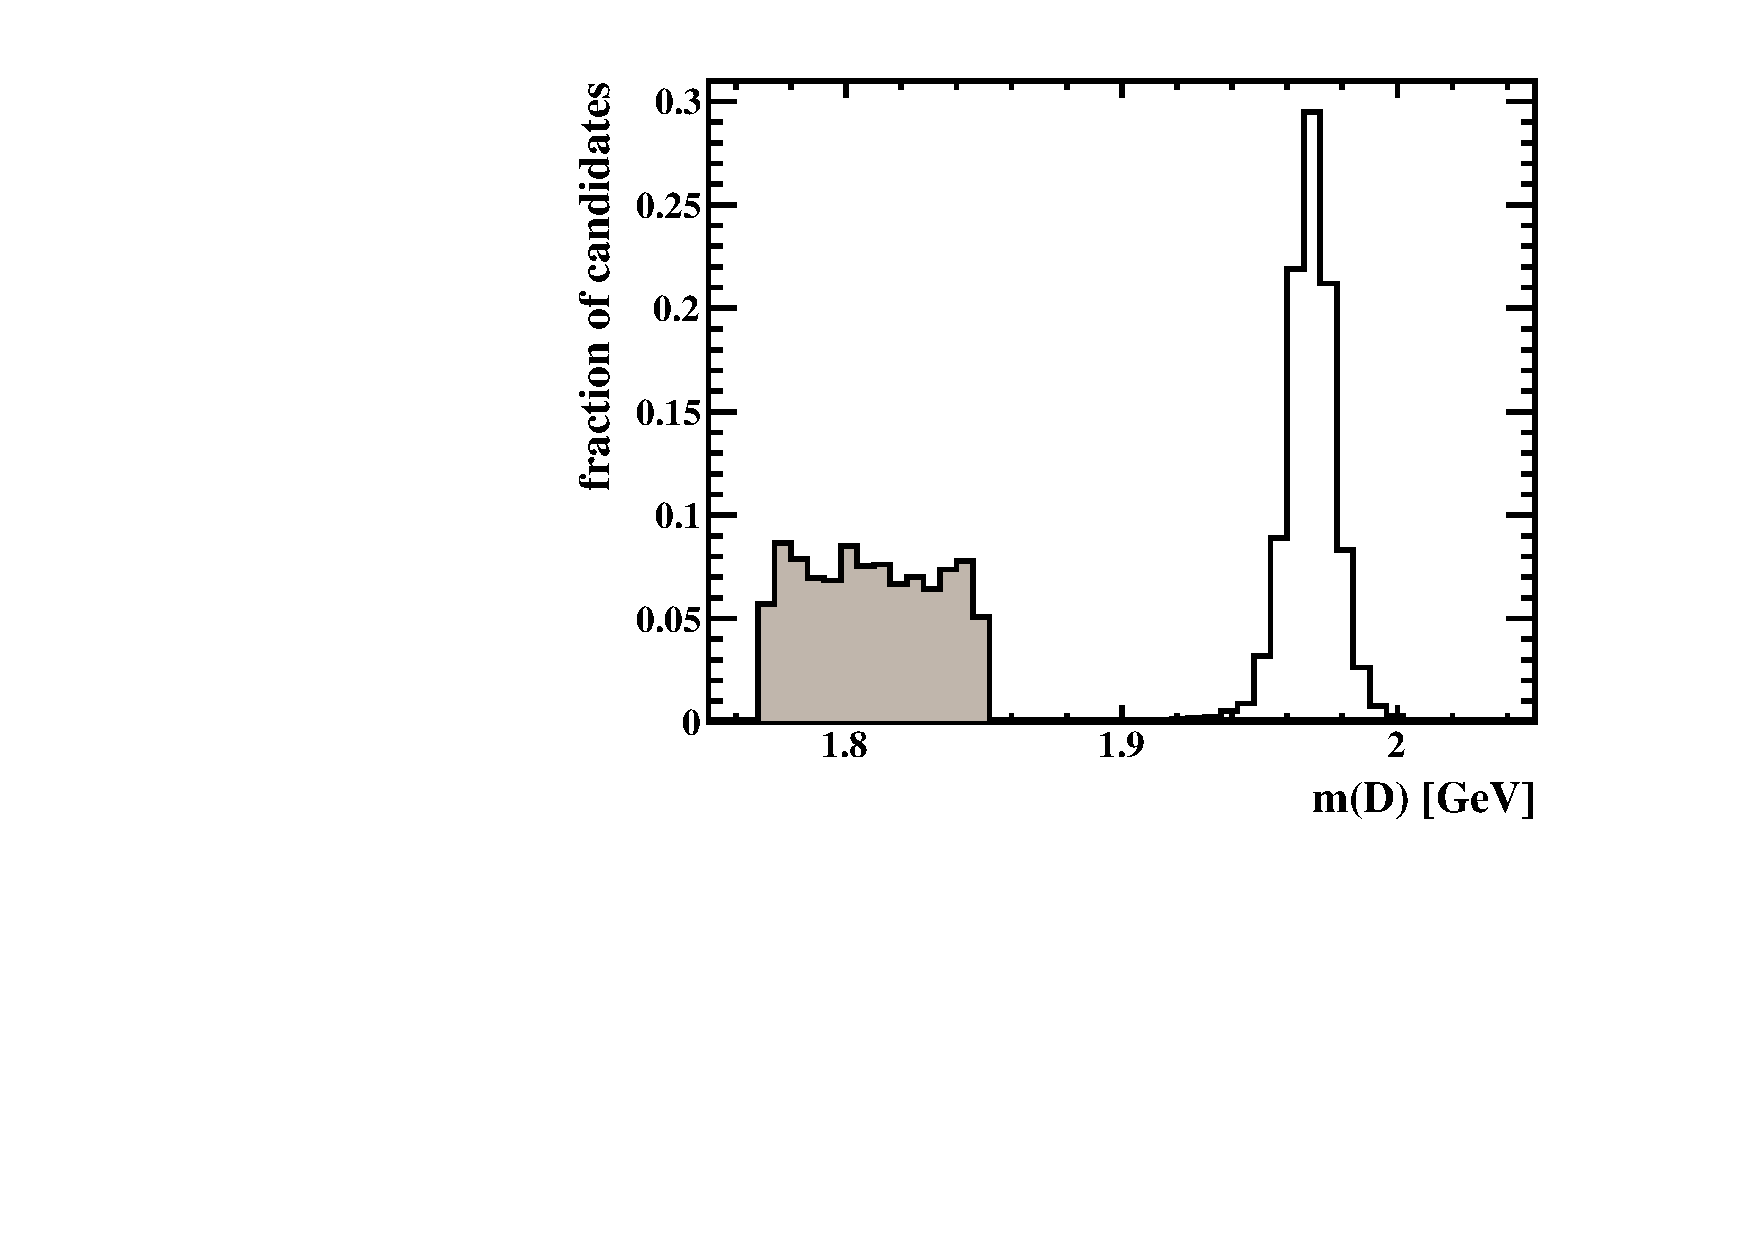
\includegraphics[width=0.49\textwidth]{../paperdraft/graphs2/mD_train.pdf}
        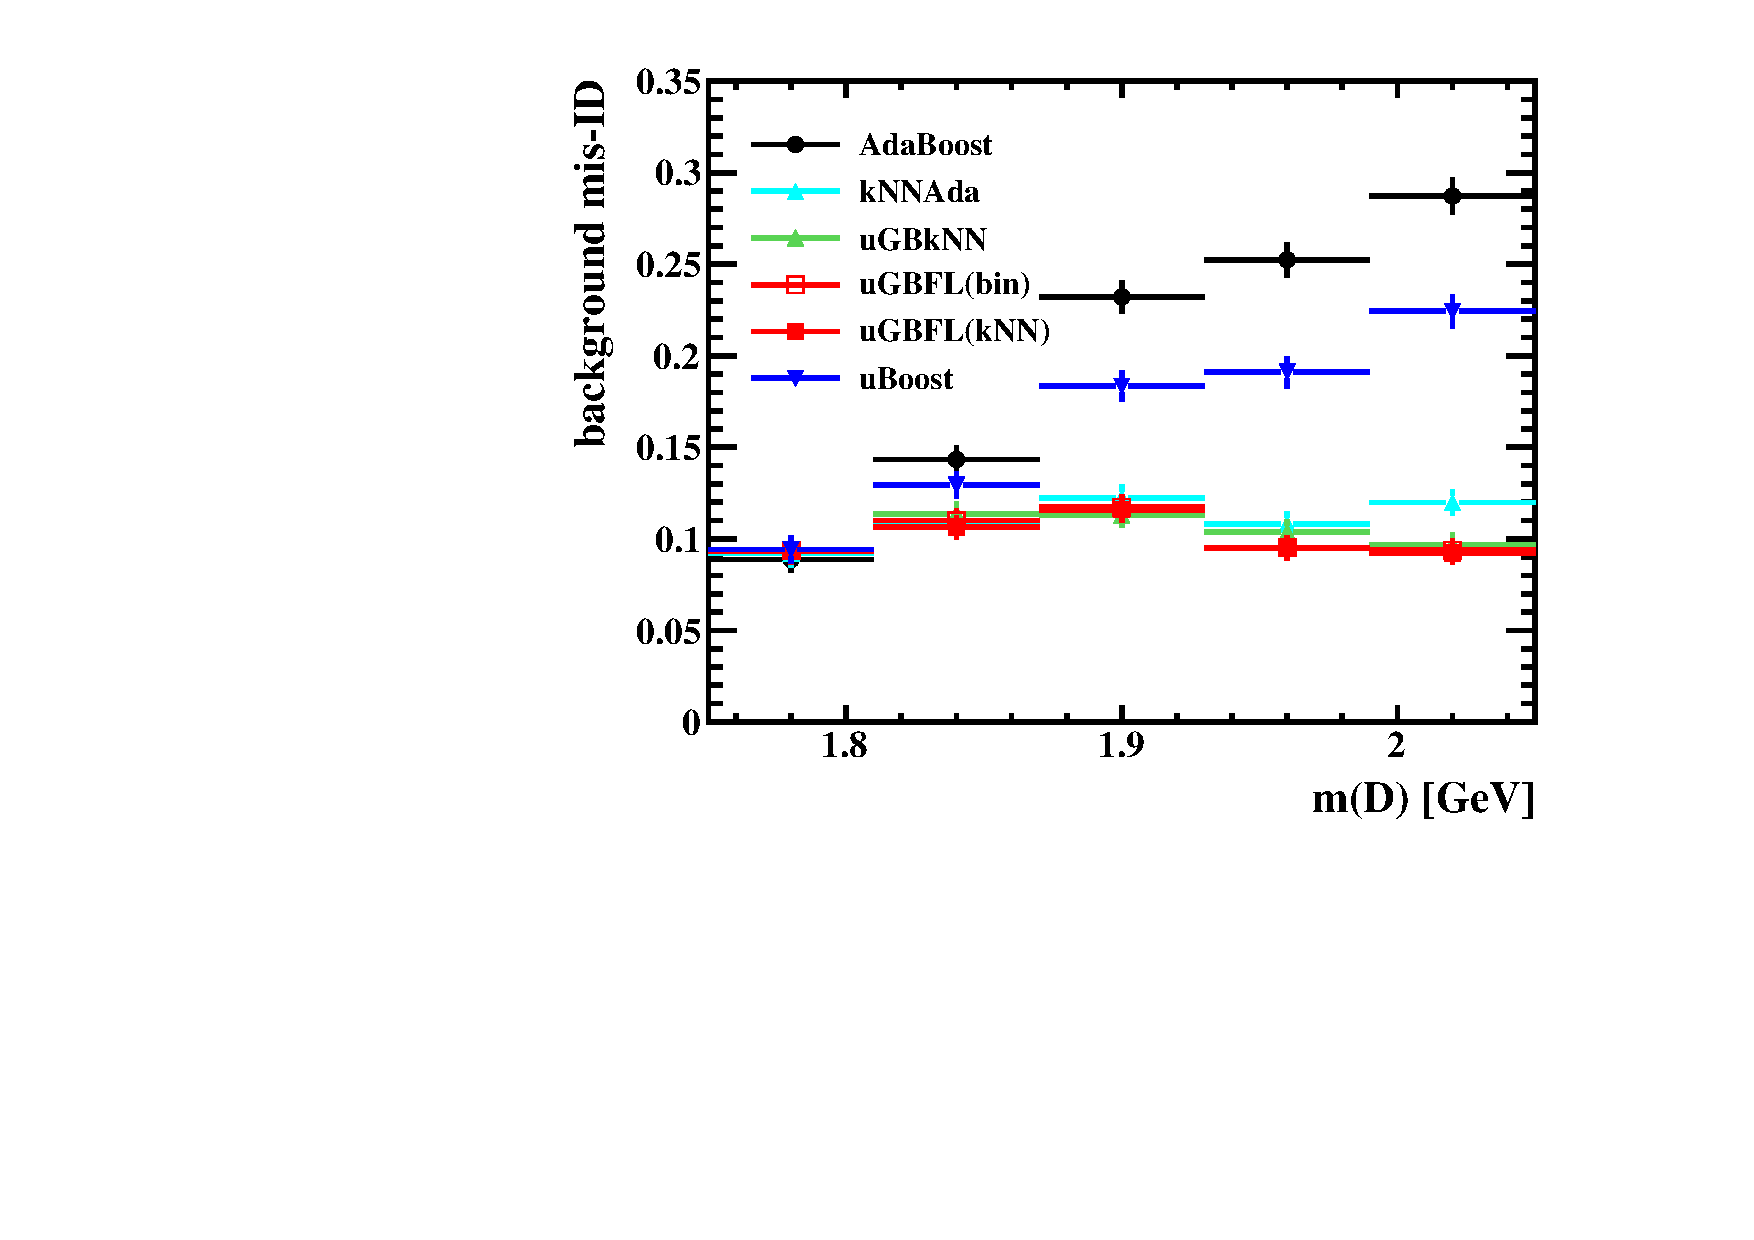
\includegraphics[width=0.49\textwidth]{../paperdraft/graphs2/MD_eff.pdf}
    \end{figure}

    (left) Signal and (filled) background samples used in training.  \\
    (right) Background mis-identification {\em vs} $D$ candidate mass for an arbitrary working point of 10\% background mis-identification in the training region $1.75 < m(D) < 1.85$~GeV is displayed.
\end{frame}


% \begin{frame}[t]
%     \frametitle{Tests on Dalitz data}
%     Testing on dataset from paper about uBoost

%     \center
%     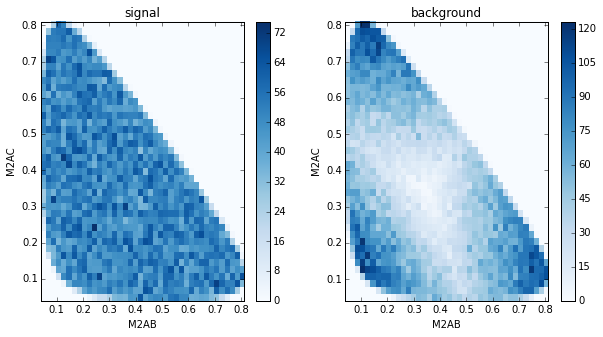
\includegraphics[width=0.6\textwidth, height=3cm]{img/dalitz_distr.png}

%     \begin{figure}
%         \centering
%         \begin{subfigure}[b]{0.48\textwidth}
%             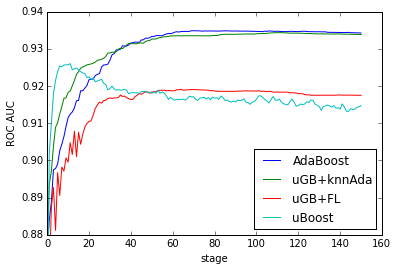
\includegraphics[width=\textwidth, height=4cm]{img/dalitz_roc_stage.png}
%             \caption{ROC vs \#trees \\ 
%              \; (greater is better)}
%         \end{subfigure}
%         \begin{subfigure}[b]{0.48\textwidth}
%             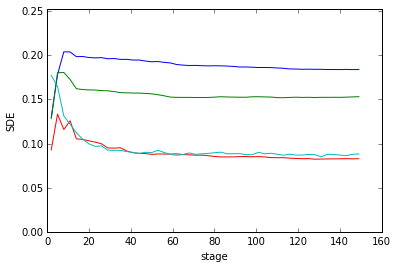
\includegraphics[width=\textwidth, height=4cm]{img/dalitz_sde.png}
%             \caption{SDE vs \#trees \\ 
%              \; (less is better)}
%         \end{subfigure}

%     \end{figure}
 % \end{frame}


% \begin{frame}[t]
%     \frametitle{Tradeoff uniformity vs quality}
%     In uGBFL we can choose different values of $alpha$ thus adjusting quality/uniformity.

%     \begin{figure}
%         \centering
%         \begin{subfigure}[b]{0.32\textwidth}
%             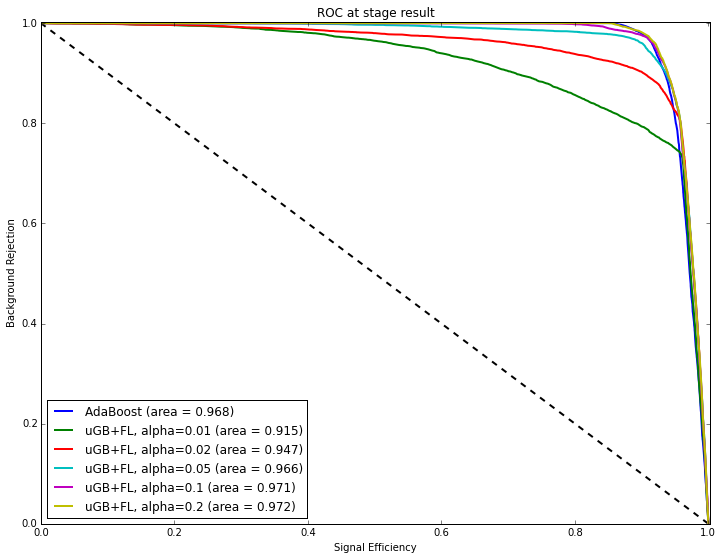
\includegraphics[width=\textwidth, height=4cm]{img/trade_roc.png}
%             \caption{ROC curves \\  
%             \; $ \;$
%             }
%         \end{subfigure}
%         \begin{subfigure}[b]{0.32\textwidth}
%             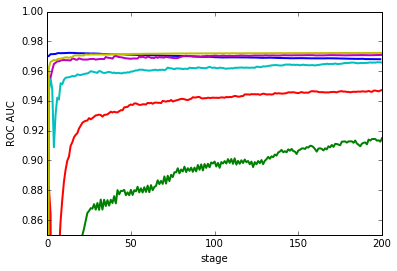
\includegraphics[width=\textwidth, height=4cm]{img/trade_roc_stage.png}
%             \caption{ROC vs \#trees \\ 
%              \; (greater is better)}
%         \end{subfigure}
%         \begin{subfigure}[b]{0.32\textwidth}
%             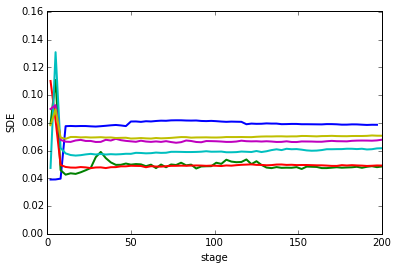
\includegraphics[width=\textwidth, height=4cm]{img/trade_sde.png}
%             \caption{SDE vs \#trees \\ 
%               \;  (less is better)
%             }
%         \end{subfigure}
%     \end{figure}
% \end{frame}


\begin{frame}[t]
    \frametitle{Summary on classifiers}
    \small
    New classifiers
    \begin{itemize}
        \item faster (than uBoost)
        \item can target at uniformity in \textit{both} signal and bck
        \item $knn$AdaBoost and gradient boosting with knnAdaLoss can be easily implemented, but don't seem to produce good uniformity
        \item uGBFL is highly tunable and proved to be able to fight severe correlation
    \end{itemize}
    $ $ \\
    uGBFL will be useful for:  
    \begin{itemize}
        \item Dalitz-plot or angular/amplitude analyses (as shown);
        \item mass measurements since both signal and background can be kept unbiased near mass peak
        \item searches for new particles since efficiency can be kept optimal for mass, lifetime values not used in the generated training samples
        \item etc
    \end{itemize}
\end{frame}


\begin{frame}
    \frametitle{Summary on metrics}
    \begin{itemize}
        \item three metrics were introduced (details in the backup)
        \item despite their difference, the results obtained with metrics proposed are \textbf{similar}.
        \item for higher dimensions: $k$-nearest neighbours modifications of metrics are available 
        {\small (instead of binning over uniform variables, we can compute nearest neighbours in the space of uniform variables).}
    \end{itemize}

Details: backup or article.
\end{frame}


\begin{frame}

    \textbf{Read}: \\
    \url{http://arxiv.org/abs/1410.4140} 
    \bigskip
    \\

    \textbf{Try out (python implementation)}: \\
    \url{https://github.com/anaderi/lhcb_trigger_ml}
    \bigskip
    \\

    Feel free to email  \\
    \url{mwill@mit.edu} \\
    \url{alex.rogozhnikov@yandex.ru} \\
    with any questions or comments.
\end{frame}



\begin{frame}
\Huge{\centerline{Q\&A}}
\end{frame}


\begin{frame}
    \Huge{\centerline{Backup}}
\end{frame}


\begin{frame}
    \frametitle{Desirable properties of metrics}
    The metric should ...
    \begin{enumerate}
    \item not depend strongly on the number of events used to test uniformity

    \item not depend on the total weight 

    \item depend on order of predictions, not the exact values of predictions \\
        (example: Pearson correlation does not satisfy this property)

    \item be stable against free parameters (number of bins, $k$ in knn)
    \end{enumerate}
\end{frame}

\begin{frame}
    \frametitle{Cut-based approach (1/2)}
    Select some set of efficiencies (in examples: 0.1, 0.3, 0.5, 0.7, 0.9), 
    for each one can compute global cut and look at efficincies in each bin:

    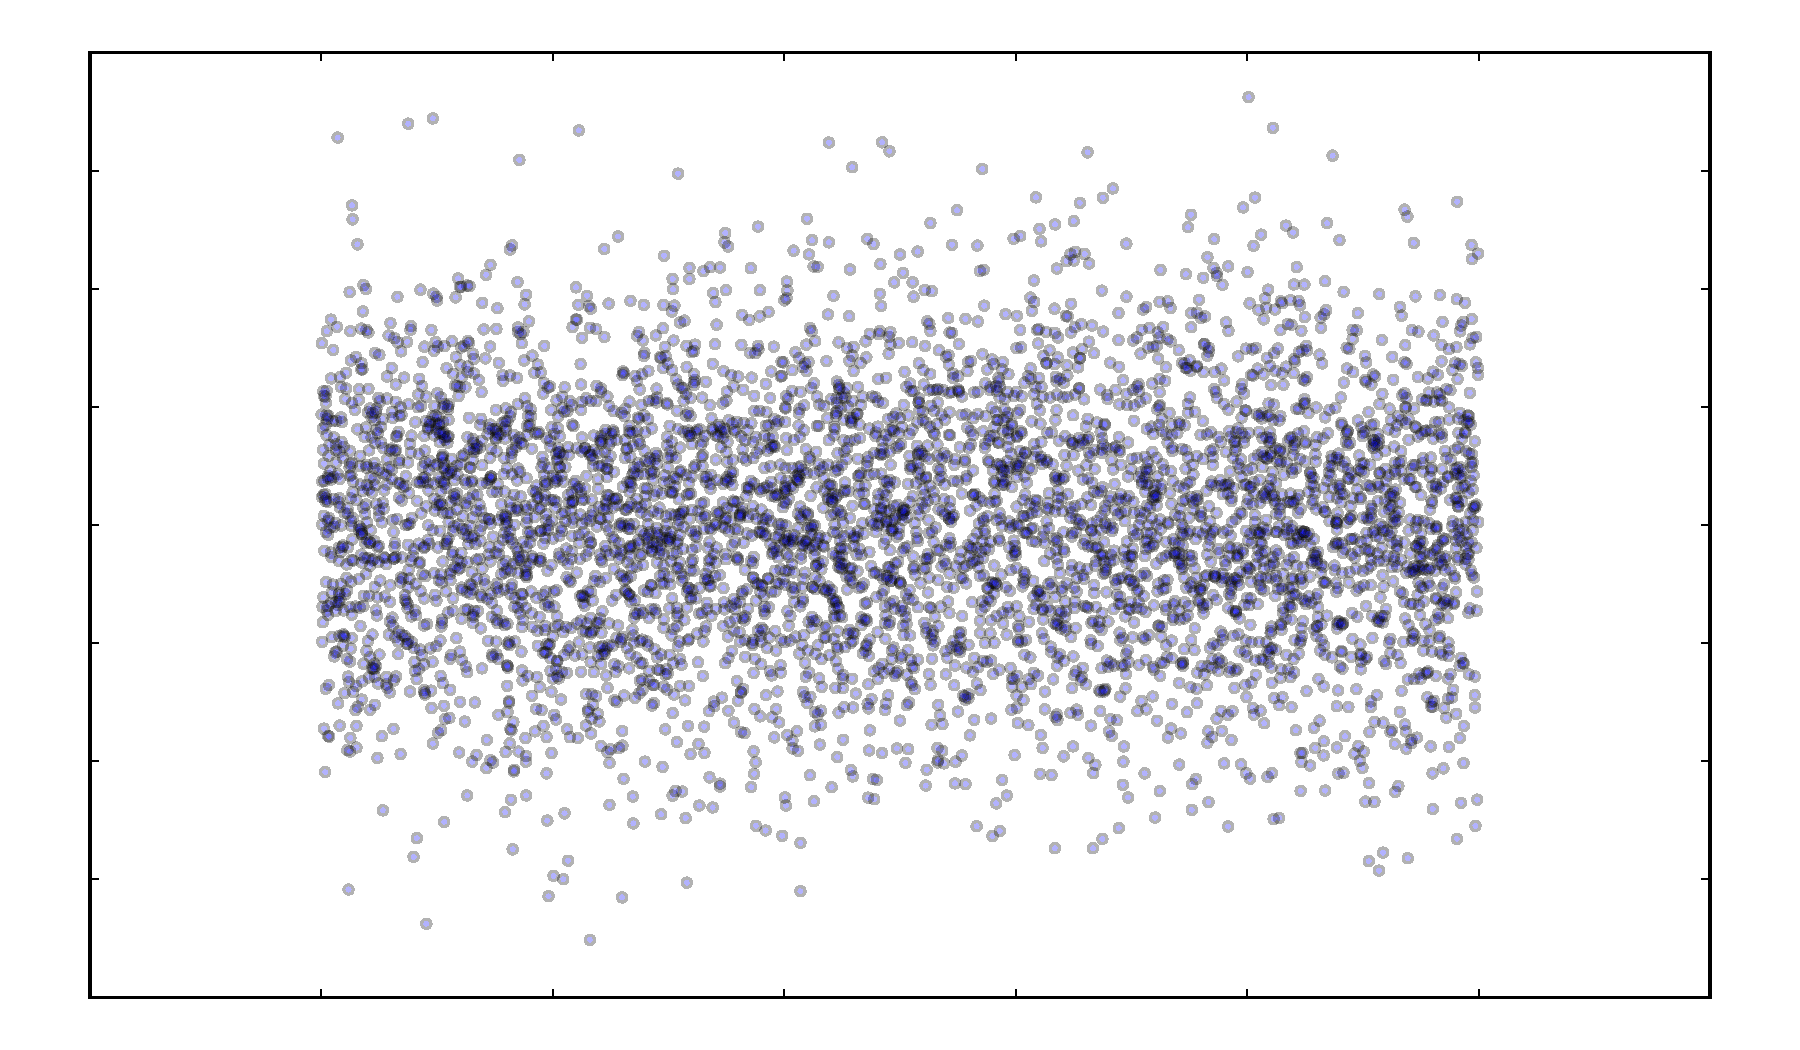
\includegraphics[width=0.5\textwidth, height=3.8cm]{img/uniform.pdf}
    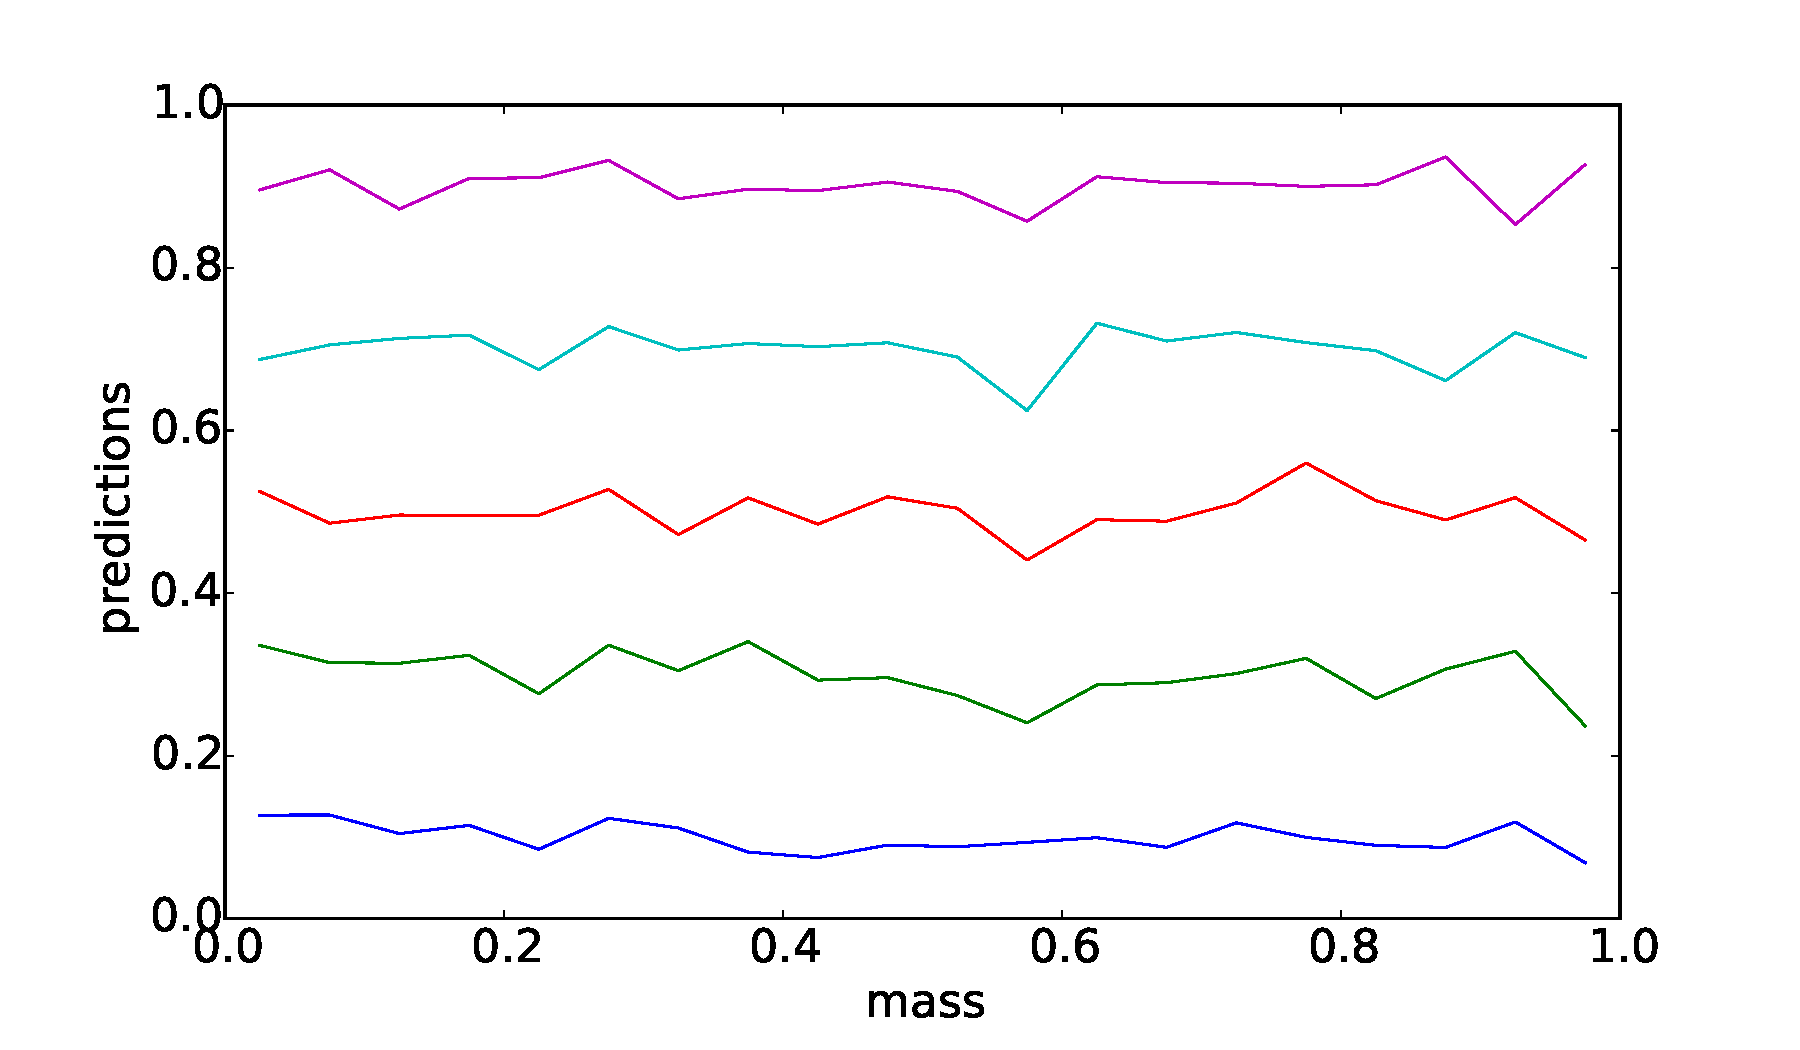
\includegraphics[width=0.5\textwidth, height=3.8cm]{img/uniform_effs.pdf}

    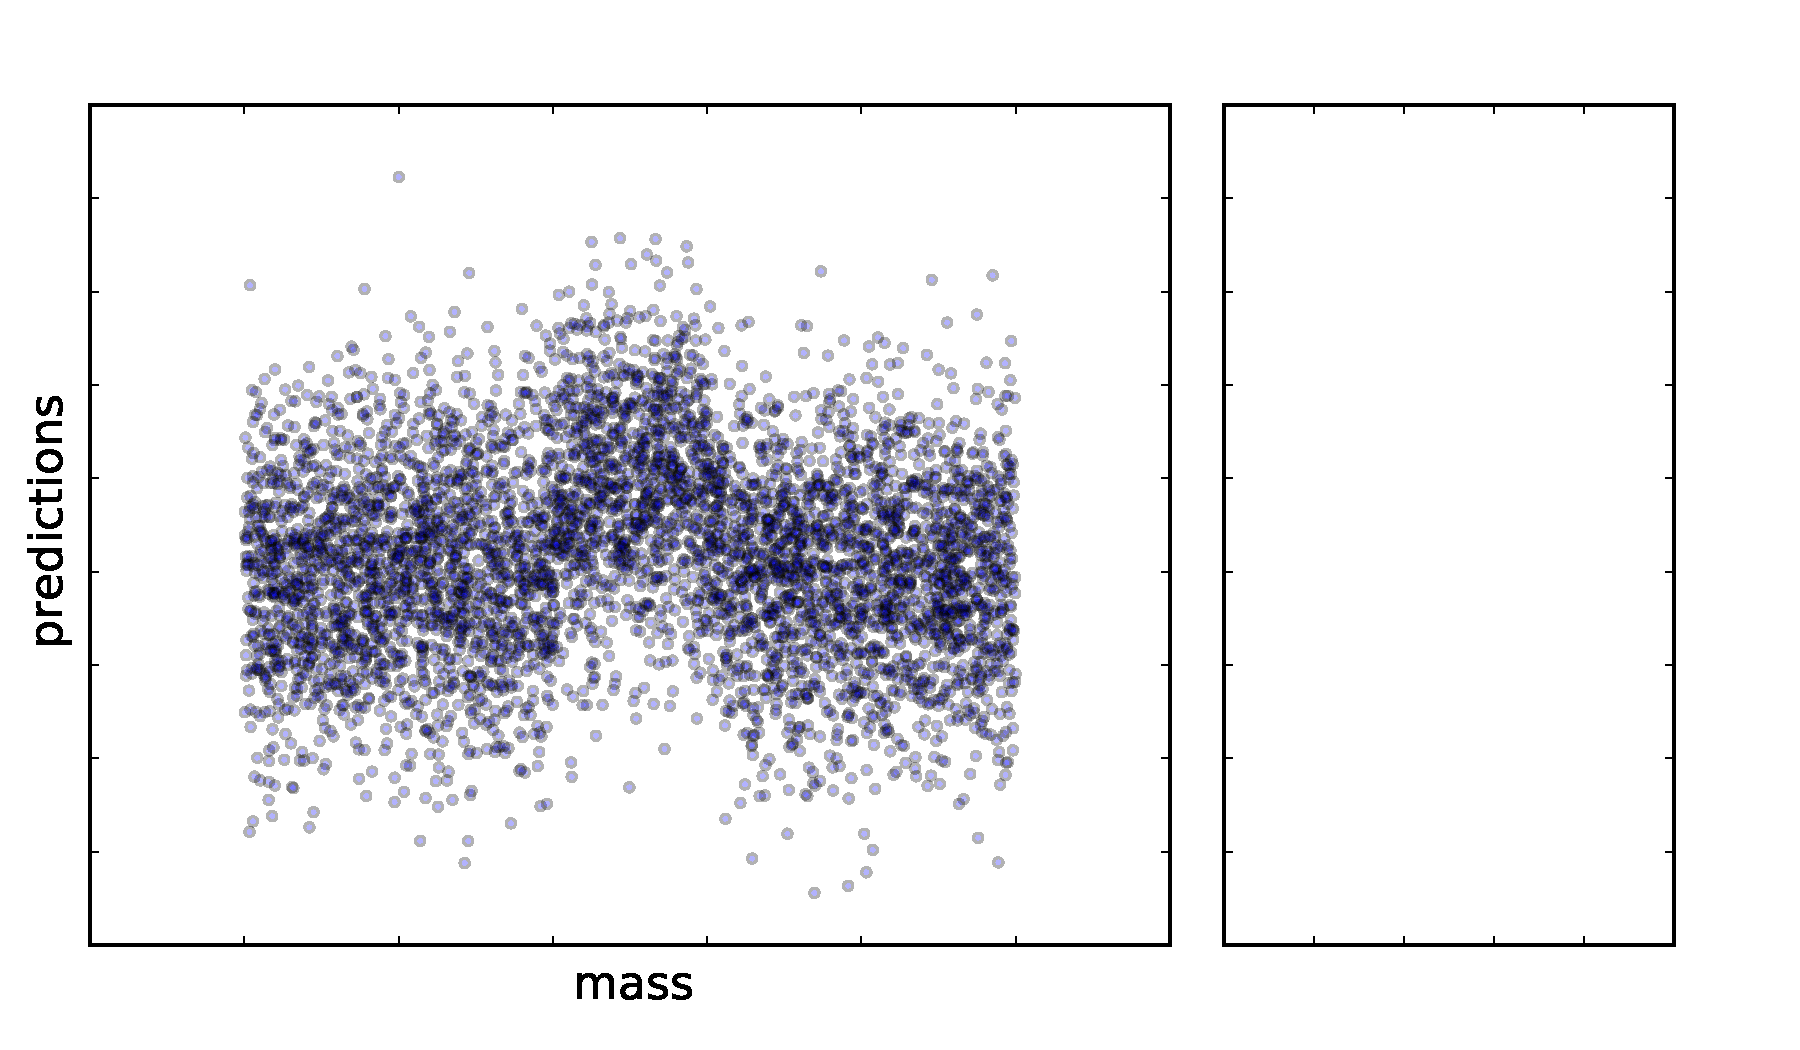
\includegraphics[width=0.5\textwidth, height=3.8cm]{img/nonuniform.pdf}
    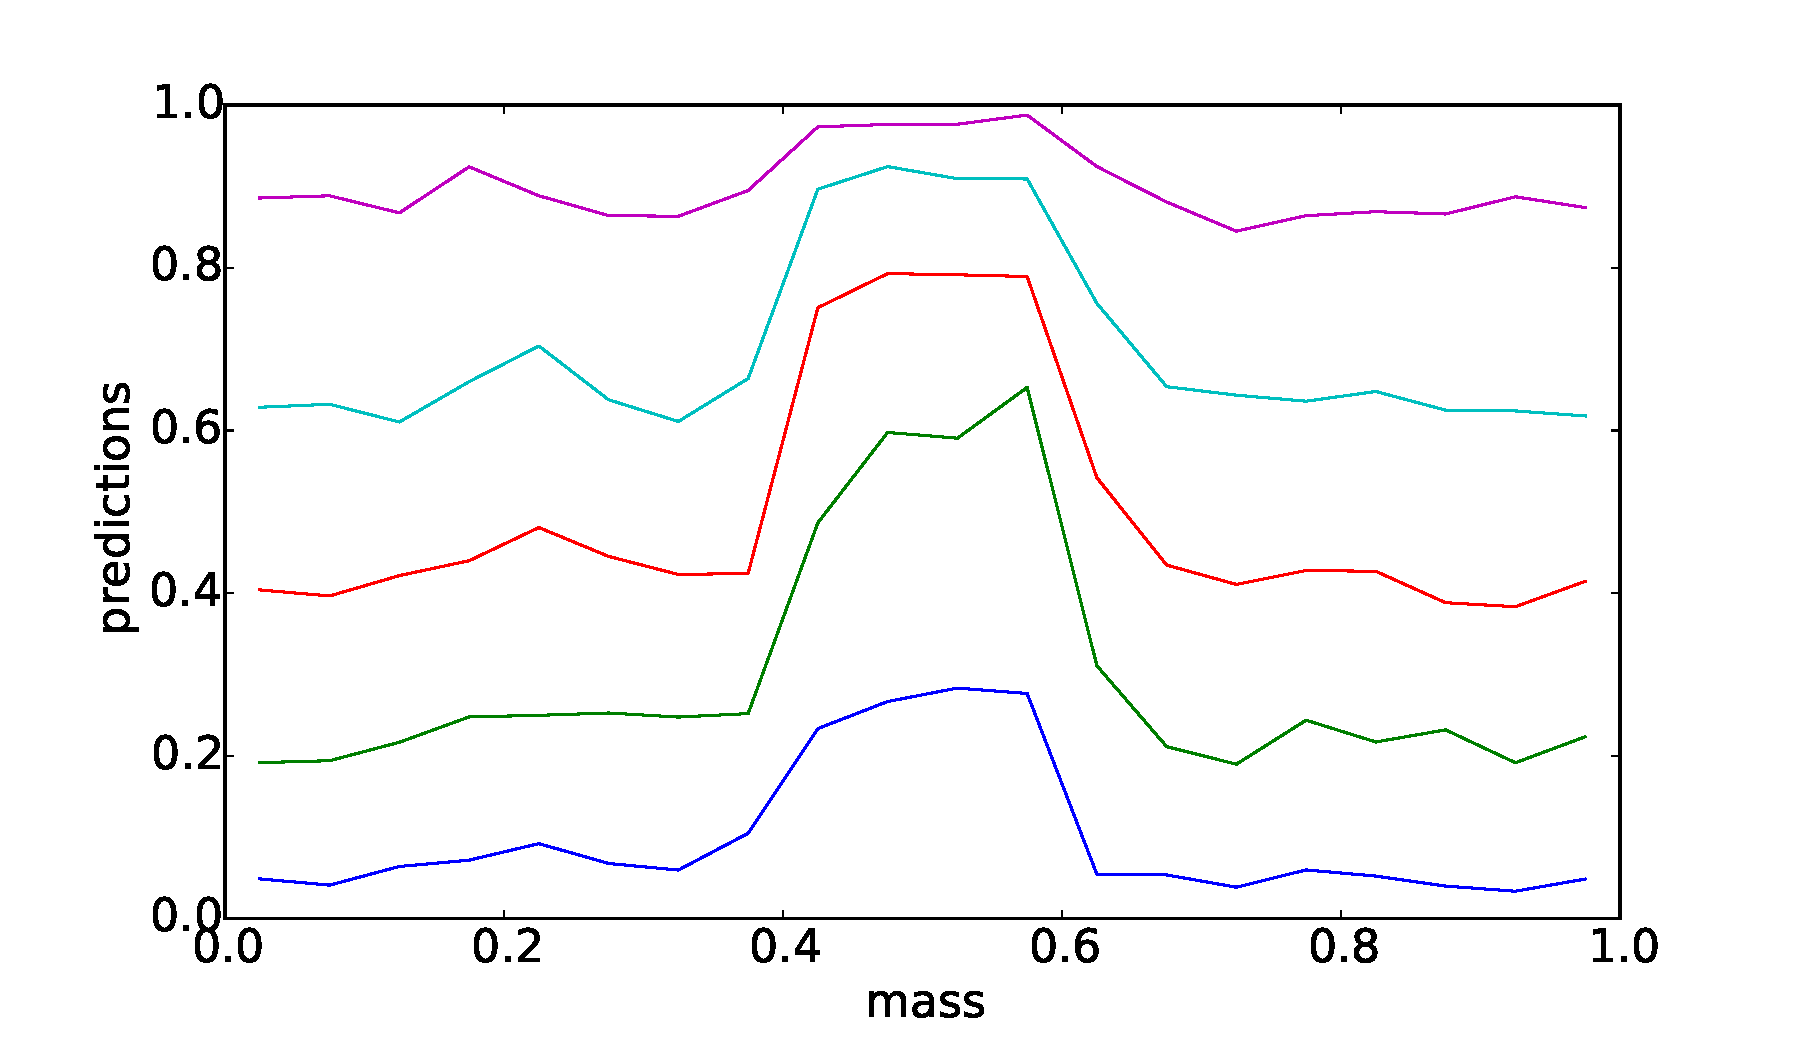
\includegraphics[width=0.5\textwidth, height=3.8cm]{img/nonuniform_effs.pdf}

\end{frame}


\begin{frame}
    \frametitle{Cut-based approach (2/2)}
    Standard deviation of efficiency
    \[
    \SDE^2(\globaleff) = 
        \sum_{\bin} \binweight \times \left(\bineff - \globaleff \right)^2 
    \]
    \[
    \SDE^2  =  \frac{1}{k} 
    \sum_{\globaleff \in [\globaleff_1 \dots \globaleff_k] }  
        \text{SDE}^2(\globaleff)
    \] 
    Theil index of $x_1, \dots, x_n$
    \[
        \theil = \frac{1}{N} \sum_i \frac{x_i}{<x>} \ln{\frac{x_i}{<x>}}, 
    \]
    Theil index of efficiency
    \[
    \theil(\globaleff) = \sum_\bin \binweight \; \frac{\bineff}{\globaleff} \; \ln{\frac{\bineff}{\globaleff}}
    \]
    \[
    \theil  =  \frac{1}{k} 
    \sum_{\globaleff \in [\globaleff_1 \dots \globaleff_k] }  
        \theil(\globaleff).
    \]
\end{frame}

\begin{frame}
    \frametitle{Example}

    {
    \centering

    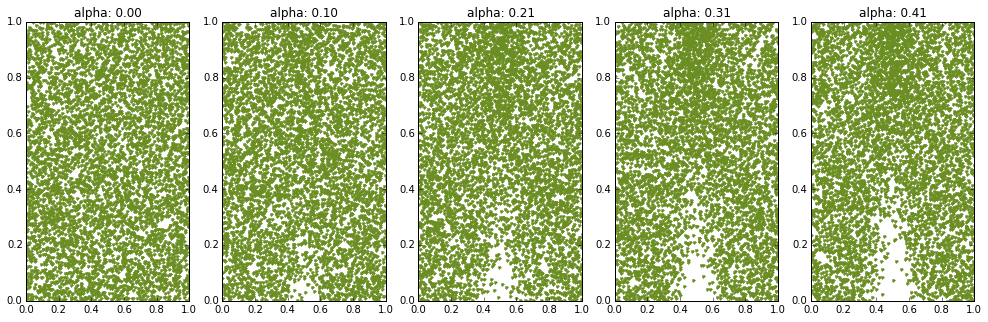
\includegraphics[width=0.9\textwidth]{img/metrics_comp1.png}

    
    \begin{figure}
    \centering

    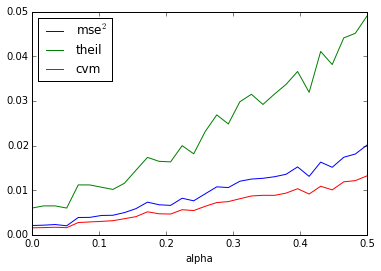
\includegraphics[width=0.5\textwidth]{img/metrics_comp2.png}
    \end{figure}
    }
\end{frame}

\begin{frame}[t]
    \frametitle{Timings of classifiers}
    One drawback of the uBoost technique is that it has a high degree of computational complexity: 
    while AdaBoost trains $M$ trees (a user-defined number), uBoost builds $100 \times M$ trees.  
    The algorithms presented only build $M$ trees; however, the boosting involves some more complicated algorithms.  Training each of the $M$ trees scales as follows for $N$ training events:
    \begin{itemize}
           \item kNNAdaBoost: $O(k \times N)$;
        \item uGBkNNknn: $O(k \times N)$ for $A_{\rm knn}$, and  
        $O( \text{\#nonzero elements in the matrix})$ for arbitrary matrix $A$;
        \item uGBFL(bin): $O(N \ln N)$;
        \item uGBFL(kNN): $O(N \ln N + N k \ln k) $.
    \end{itemize}

    Usually the training time for these new algorithms is within a factor of two the same as AdaBoost.  

\end{frame}

\end{document}